\documentclass[10pt]{article}
\usepackage{graphicx}
\usepackage{subcaption}
\usepackage[T1]{fontenc}
\usepackage{amsmath}
\usepackage{lipsum}
\usepackage{hyperref}
\usepackage[utf8]{inputenc}
\usepackage[letterpaper,margin=1in]{geometry}
\usepackage[parfill]{parskip}
\usepackage[europeanresistors, american]{circuitikz}
\usetikzlibrary{arrows,shapes,calc,positioning}
\usetikzlibrary{shapes}
\usetikzlibrary{plotmarks}

\newcommand{\oscope}[2] % #1 = name , #2 = rotation angle
{
    \draw[thick,rotate=#2] (#1) circle (12pt)
    (#1) ++(-0.35,-0.1) -- ++(0.3,0.3) --++(0,-0.3)-- ++(0.3,0.3) --++(0,-0.3);
}

\vspace{-8ex}
\date{}
\begin{document}

\title{\textbf{\Large{\textsc{ECE320:} Fields and Waves}} \\ \Large{Lab 1 Report: Waves on Transmission Lines} \\ \textbf{\small{PRA106}}\vspace{-0.3cm}}
\author{Alp Tarım, Pranshu Malik \\ \footnotesize{1003860128}, \footnotesize{1004138916}}

\maketitle

\section{Introduction}

This laboratory focused on investigating the characteristics of transmission lines, studying voltage and current 
propagation along them, as well as its depedance on the nature of load impedance.

\section[Determining the Characteristic Impedance, Z0]{Determining the Characteristic Impedance, {$Z_0$}}

We varied the load on the switch box until we saw little or no traces of reflected waves.
This was at $Z_L = 50 \Omega$ which is also equal to the charactertic impedance 
since we know that the reflections nullify when $Z_L = Z_0$. The corresponding waveforms
captured at the generator input (channel 1, top) and the transmission line input (channel 2, bottom) 
are shown in Figure 1.

\begin{figure}[h]
    \centering
    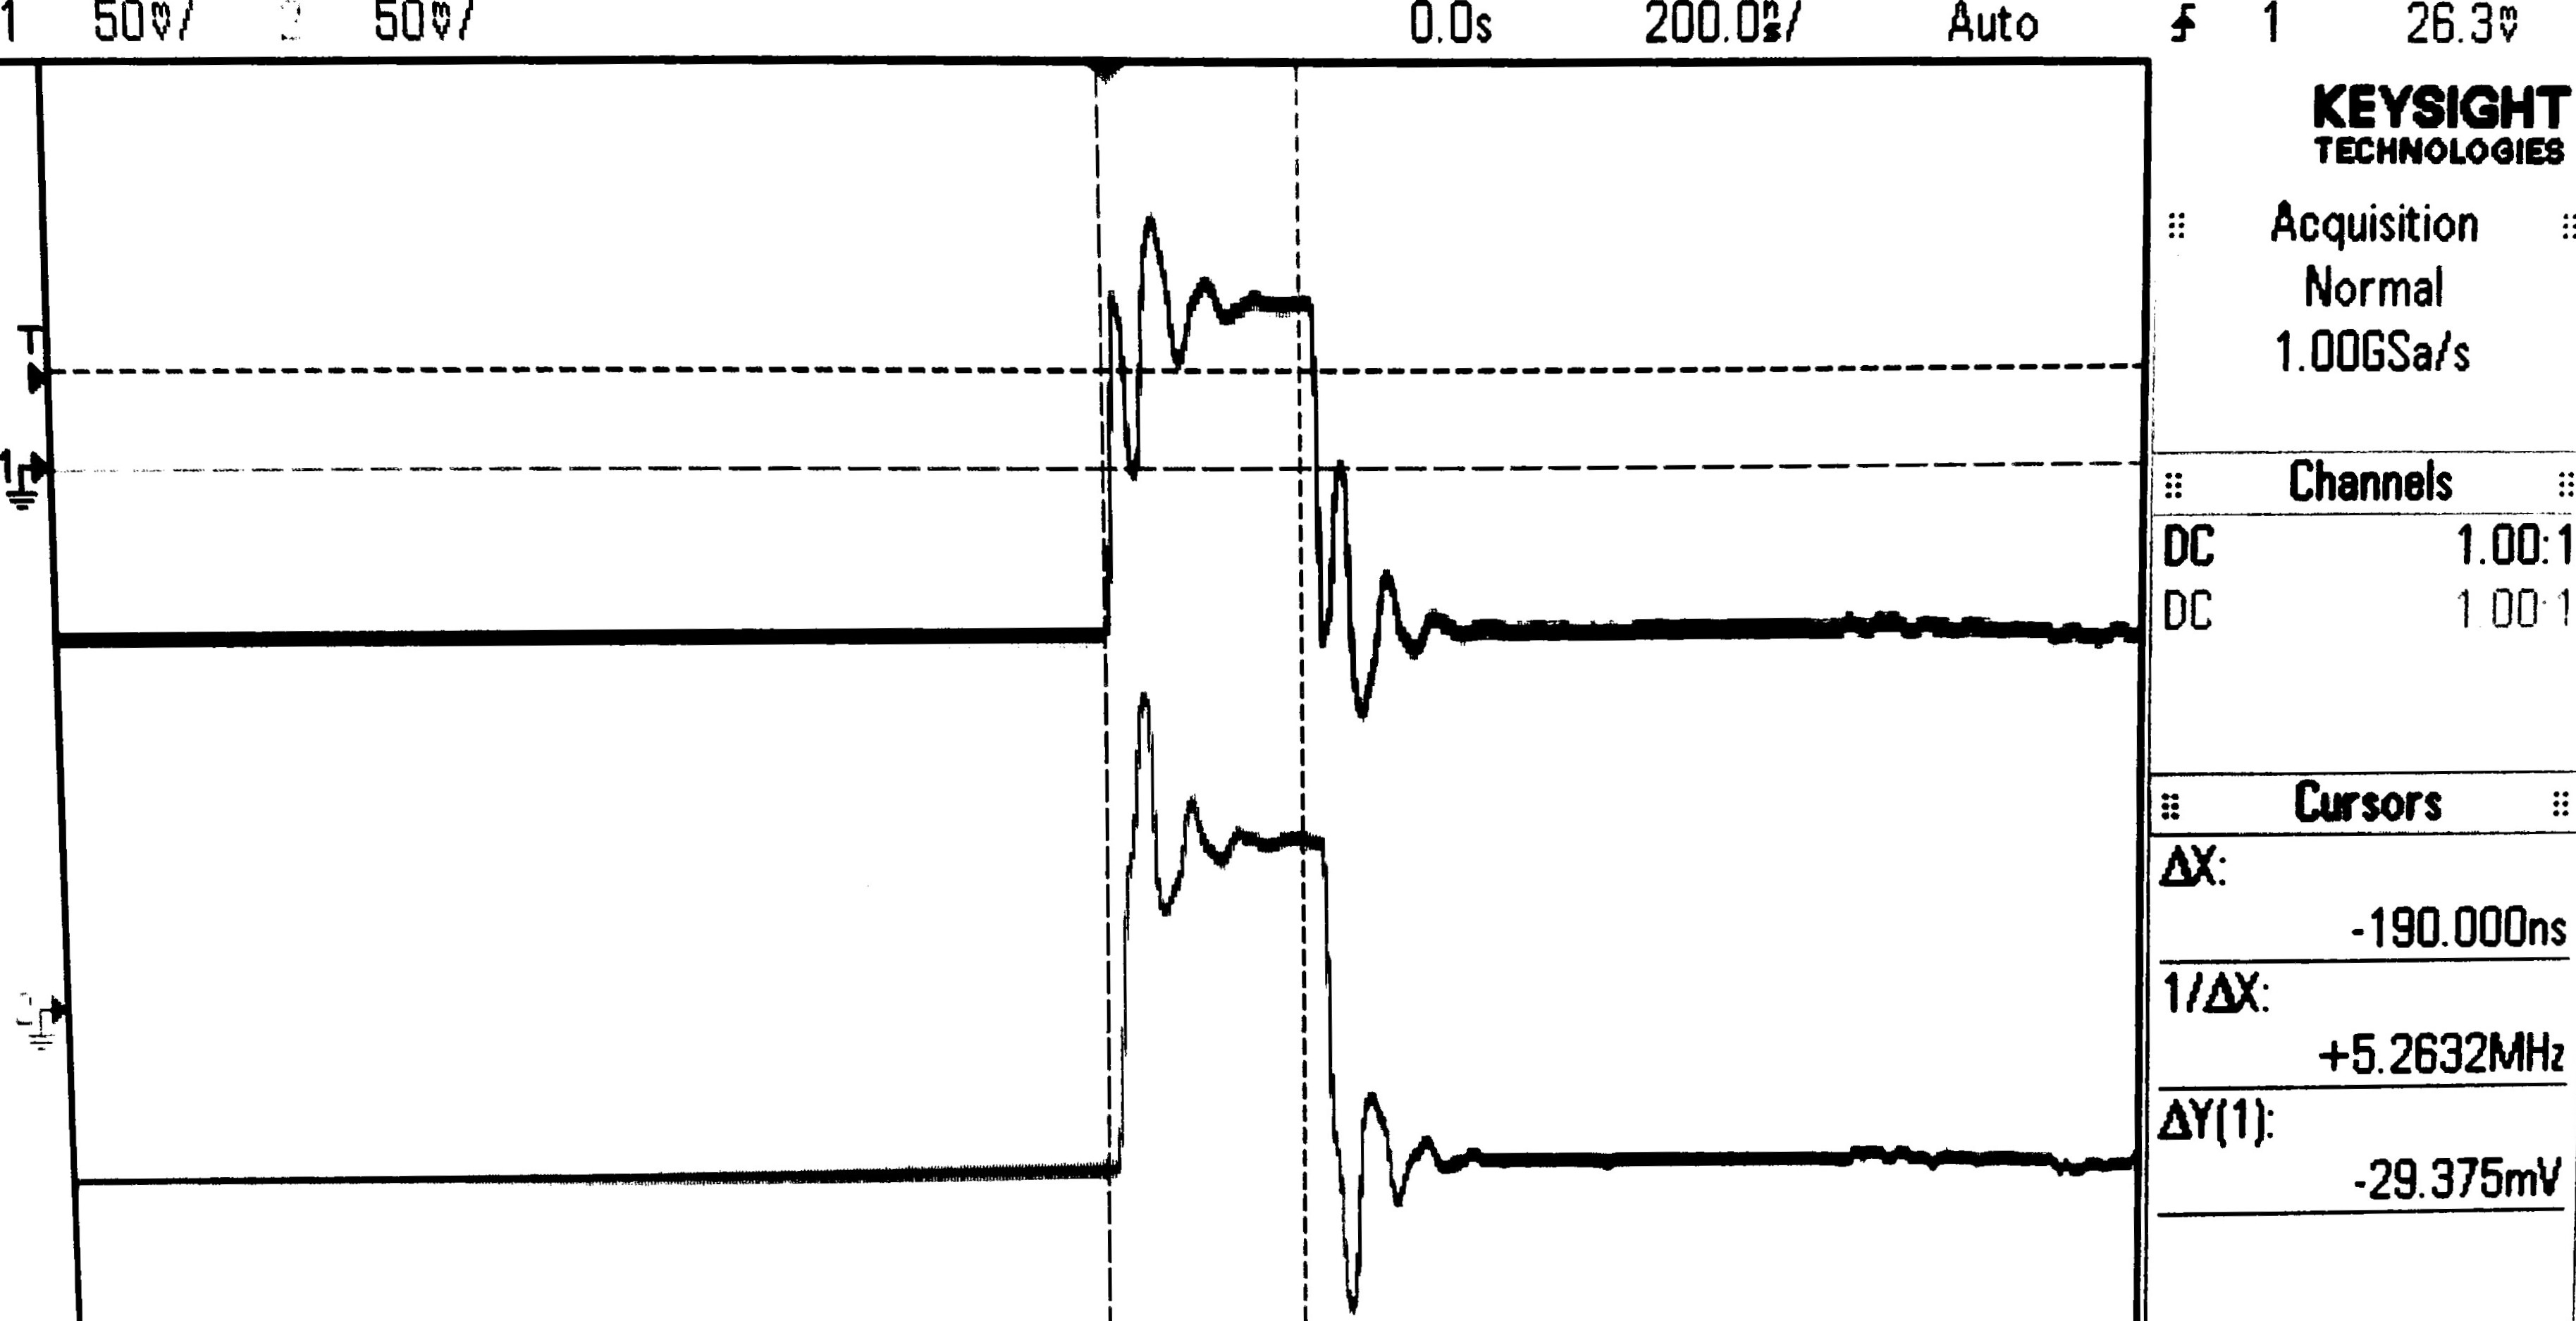
\includegraphics[width=0.45\textwidth]{../photos/lab1/load_matched.jpg}
    \caption{Transmission line terminated with load $Z_L = Z_0$\vspace{-0.5cm}}
    \label{tline_matching_z_0}
\end{figure}

\section[Determining Z0 using V/I]{Determining $Z_0$ using $\frac{\tilde V^+(z=-L)}{\tilde I^+(z=-L)}$}

\begin{figure}[ht] \centering
    \begin{circuitikz} 
        \draw
        (0,2) to [sqV, l_=$\tilde V_g$] (0, 0) -- (2,0)
        to [tline, l_=Transmission Line, o-o] (7,0)
        to [R, l=$Z_L$] (7, 2)
        to [tline, l=${Z_0, \beta, L}$, o-o] (2,2)
        to [R, l_=$Z_g$, i<^=$\tilde I$] (0, 2);
        
        \draw (2,2.35) node{$\tilde V$} (2, 2);
        \draw (2,0) -- (2.5,-0.15) to[sV, l_=\footnotesize{CH1}, color=white, name=CH1] (2.5,1.75) -- (2, 2);
        \oscope{CH1}{0}
        \draw (7,0) -- (8,-0.15) to[sV, l_=\footnotesize{CH2}, color=white, name=CH2] (8,1.75) -- (7, 2);
        \oscope{CH2}{0}
        \draw (0,0) to[short, *-*] node[ground]{} (0,0);
        \draw [dotted] (2,-0.35) -- (2,0.35) (7,-0.35) -- (7,0.35)
        (2.1, -0.5) node{$z=-L$} (2, -0.35) (7, -0.5) node{$z=0$} (7, -0.35);
    \end{circuitikz}
    \caption{Laborartory setup for studying characteristcs of tranmission lines\vspace{-0.5cm}}
    \label{tline_diag}
\end{figure}

\begin{figure}[ht]
    \centering
    \begin{subfigure}[b]{0.45\textwidth}
        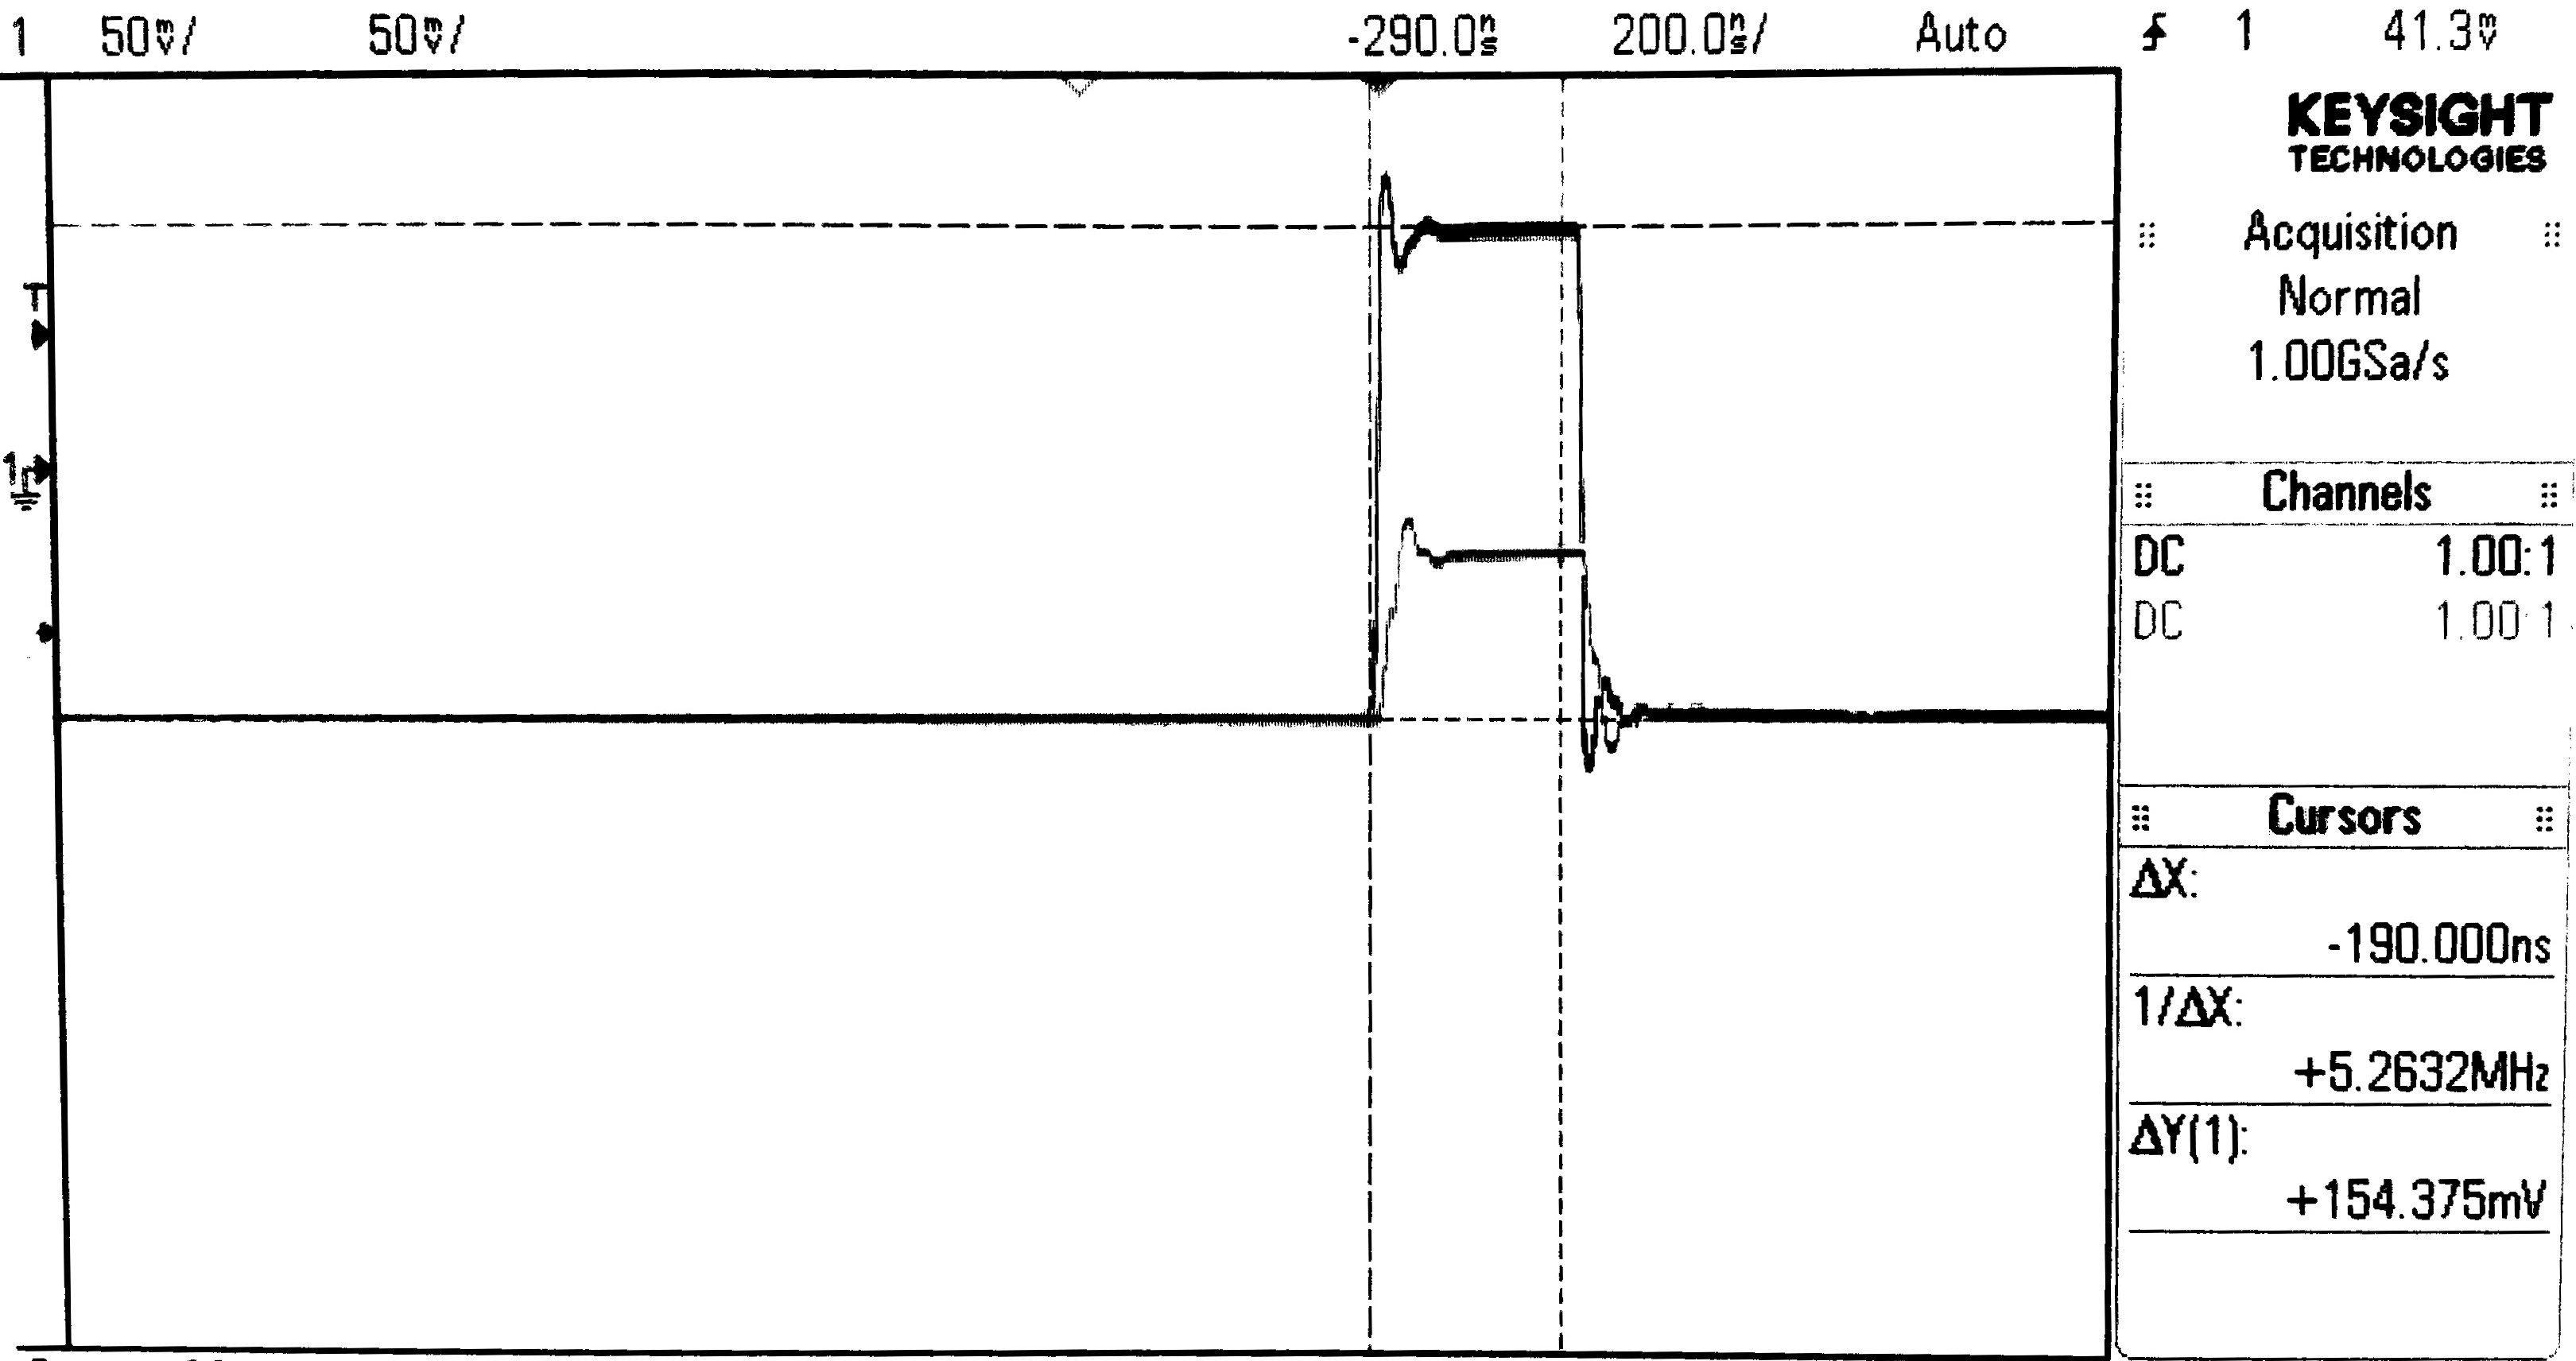
\includegraphics[width=\textwidth]{../photos/lab1/shunt_delta_v_1.jpg}
        \caption{$\tilde V_1 \approx 154\text{mV}$}
    \end{subfigure}
    \quad
    \begin{subfigure}[b]{0.45\textwidth}
        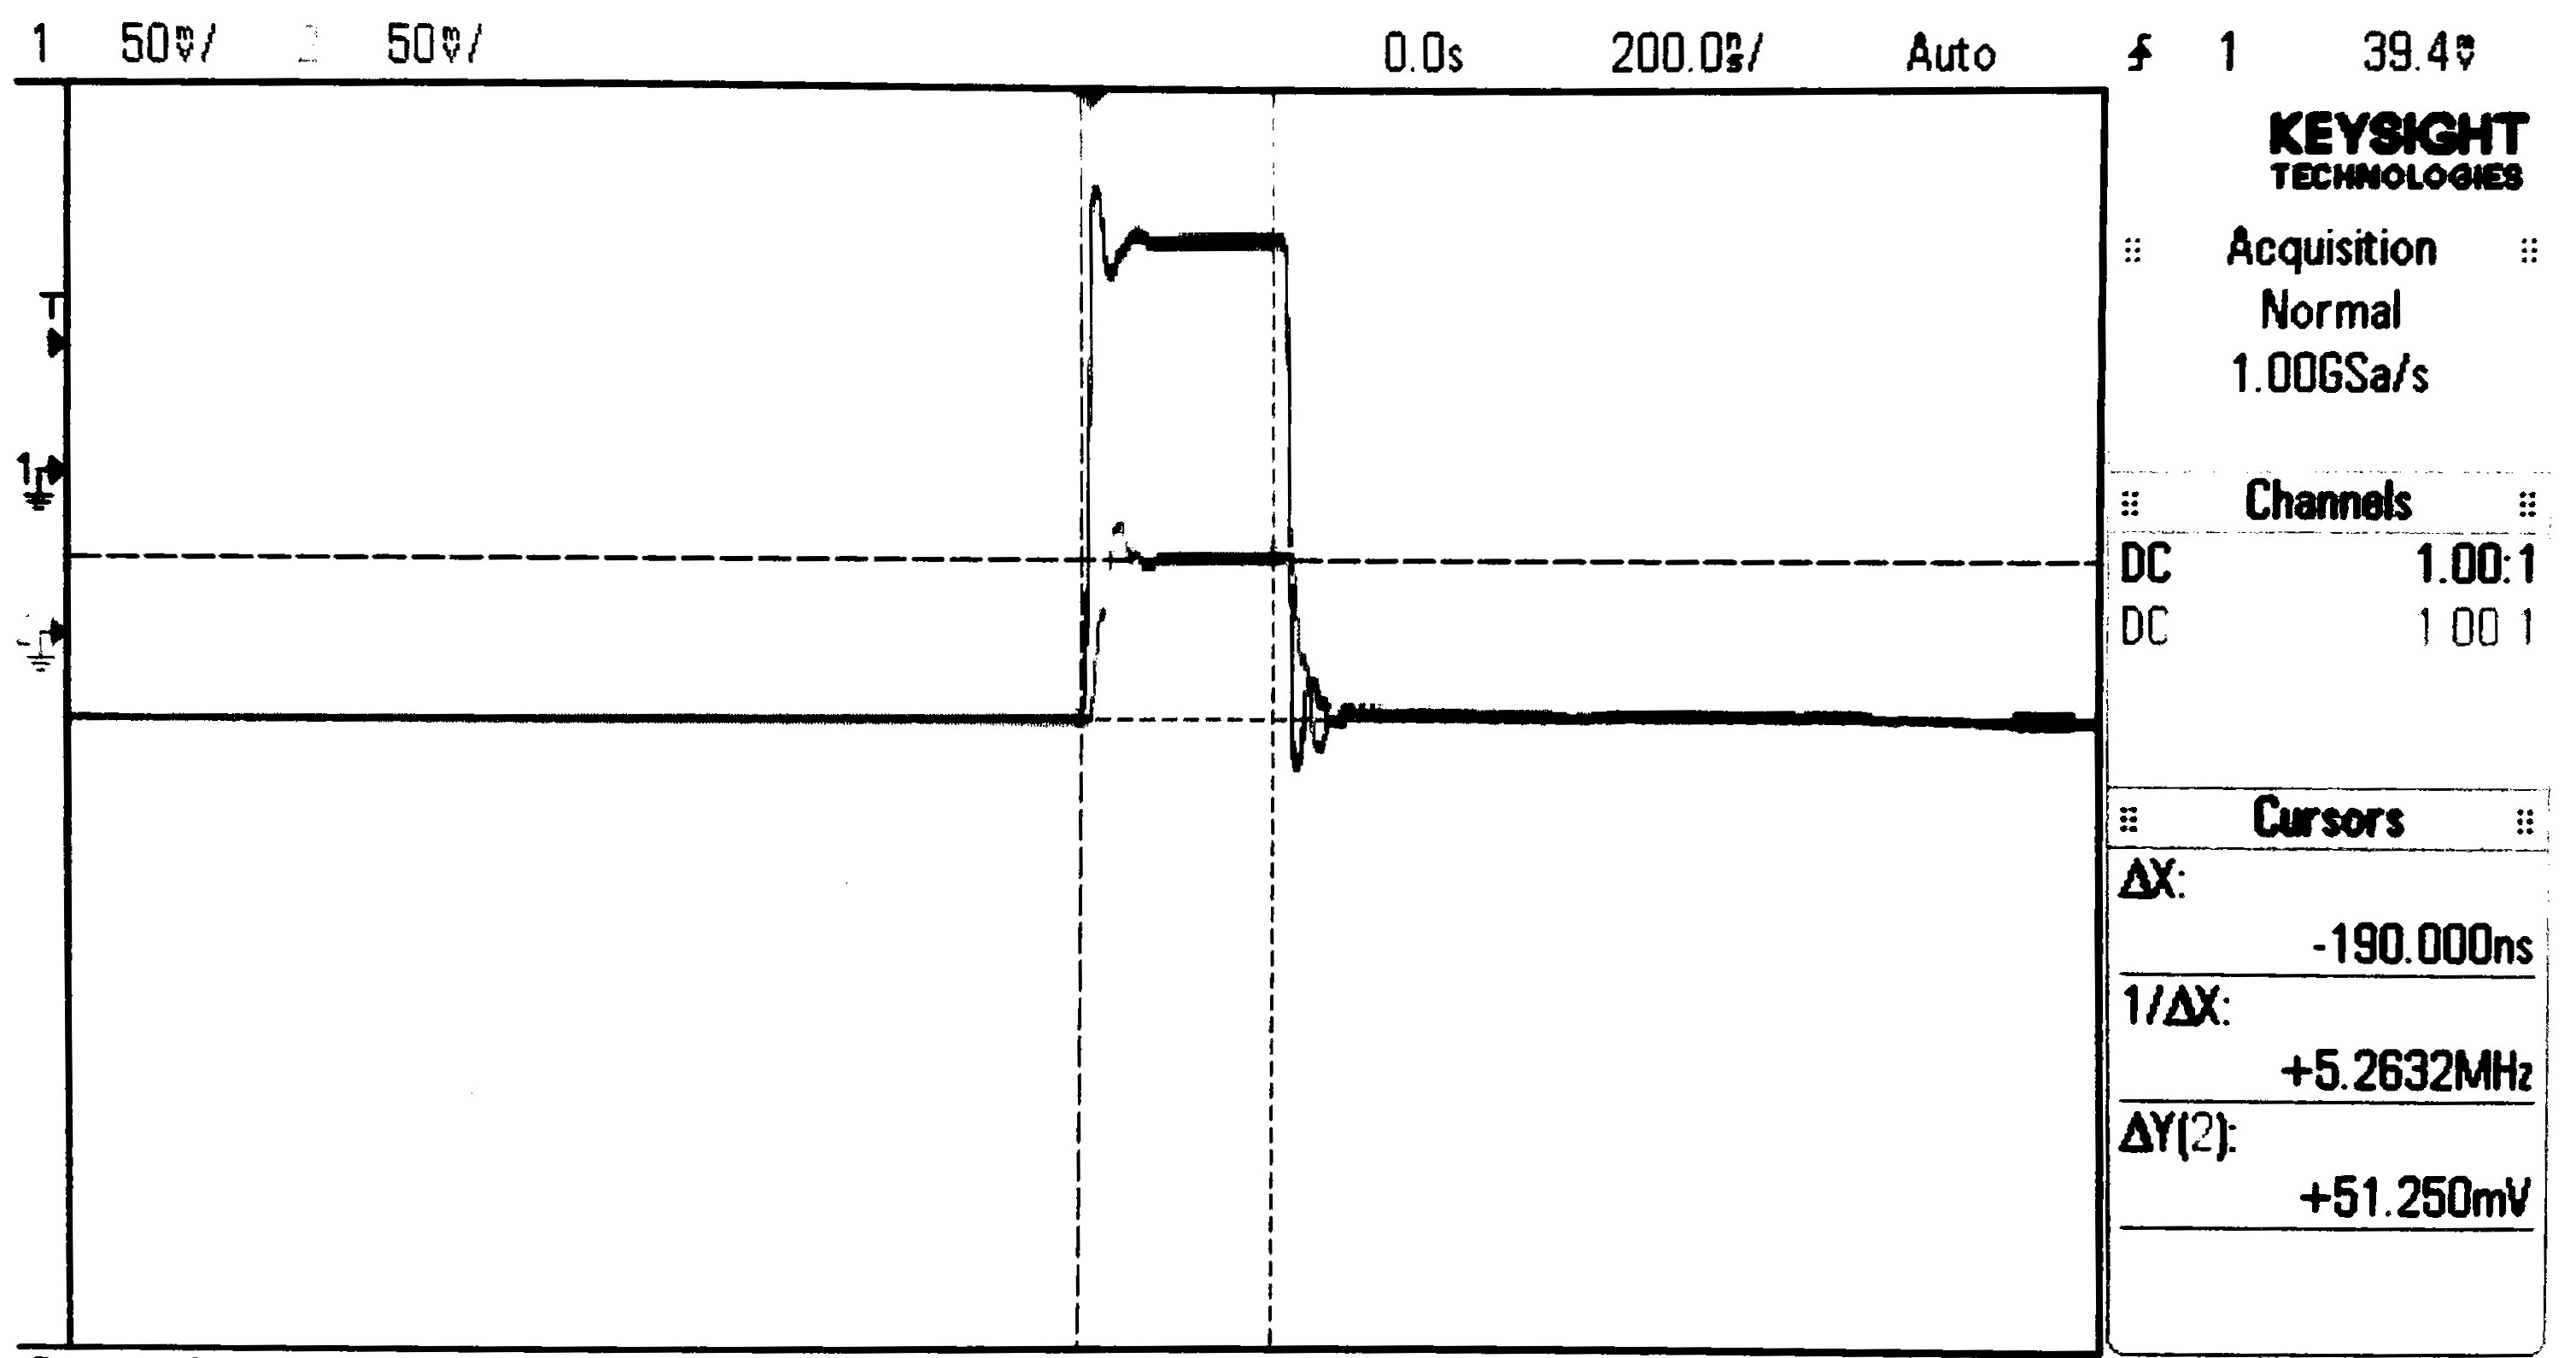
\includegraphics[width=\textwidth]{../photos/lab1/shunt_delta_v_2.jpg}
        \caption{$\tilde V_2 \approx 51\text{mV}$}
    \end{subfigure}
    \caption{$\tilde V$ measured across $R_\text{shunt} = 100\Omega$\vspace{-0.5cm}}
    \label{delta_v_shunt}
\end{figure}

As seen in Figure 3, the voltage at $\tilde V_1 = 154\text{mV}$ and $v_1 = 51\text{mV}$. Given the value of $R_\text{shunt} = 100\Omega$,
we can calculate $\tilde I^+ = \frac{0.154-0.051}{100} = 1.03\text{mA}$. From Figure 4, we can see that $\tilde V_2 = \tilde V^+$, and therefore we can confirm the
value of $Z_0$ through the relation, $Z_0 := \frac{\tilde V^+(z=-L)}{\tilde I^+(z=-L)} = \frac{51\text{mV}}{1.03\text{mA}} = 49.51\Omega \approx 50\Omega$.

\begin{figure}[h] \centering
    \begin{circuitikz} 
        \draw [dotted][thick] (0,0) -- (0,2) (2,0) -- (2,2) (0, 2) -- (-1, 2) (2, 2) -- (3, 2);
        \draw (0,1.5) to [R, l=$R_{\text{shunt}}$, i>^=$\tilde I$, *-*] (2, 1.5);
        \draw (0,0.15) -- (2, 0.15);
        \draw (1, 0.15) to [short, *-*] node[ground]{} (1,0.15);
        \draw (0,0.15) circle (1.5pt);
        \draw (2,0.15) circle (1.5pt);
        \draw (2,0.15) -- (2.5,-0.15) to[sV, l_=$\tilde V_2$, color=white, name=CH2] (2.5,1.35) -- (2, 1.5);
        \oscope{CH2}{0}
        \draw (0,0.15) -- (-0.5,-0.15) to[sV, l=$\tilde V_1$, color=white, name=CH1] (-0.5,1.35) -- (0, 1.5);
        \oscope{CH1}{0}

        \draw (4.75,1) node[]{$\displaystyle{\tilde I = \frac{\tilde V_1 - \tilde V_2}{R_{\text{shunt}}}}$} (4.75,1);
    \end{circuitikz}
    \caption{Estimating input current through a shunt resistance \vspace{-0.5cm}}
    \label{shunt_diag}
\end{figure}

\section{Observation of Travelling Waves}

Observed waveforms at different points on the transmission line can be found in Figure 5.

\begin{figure}[ht]
    \centering
    \begin{subfigure}[b]{0.45\textwidth}
        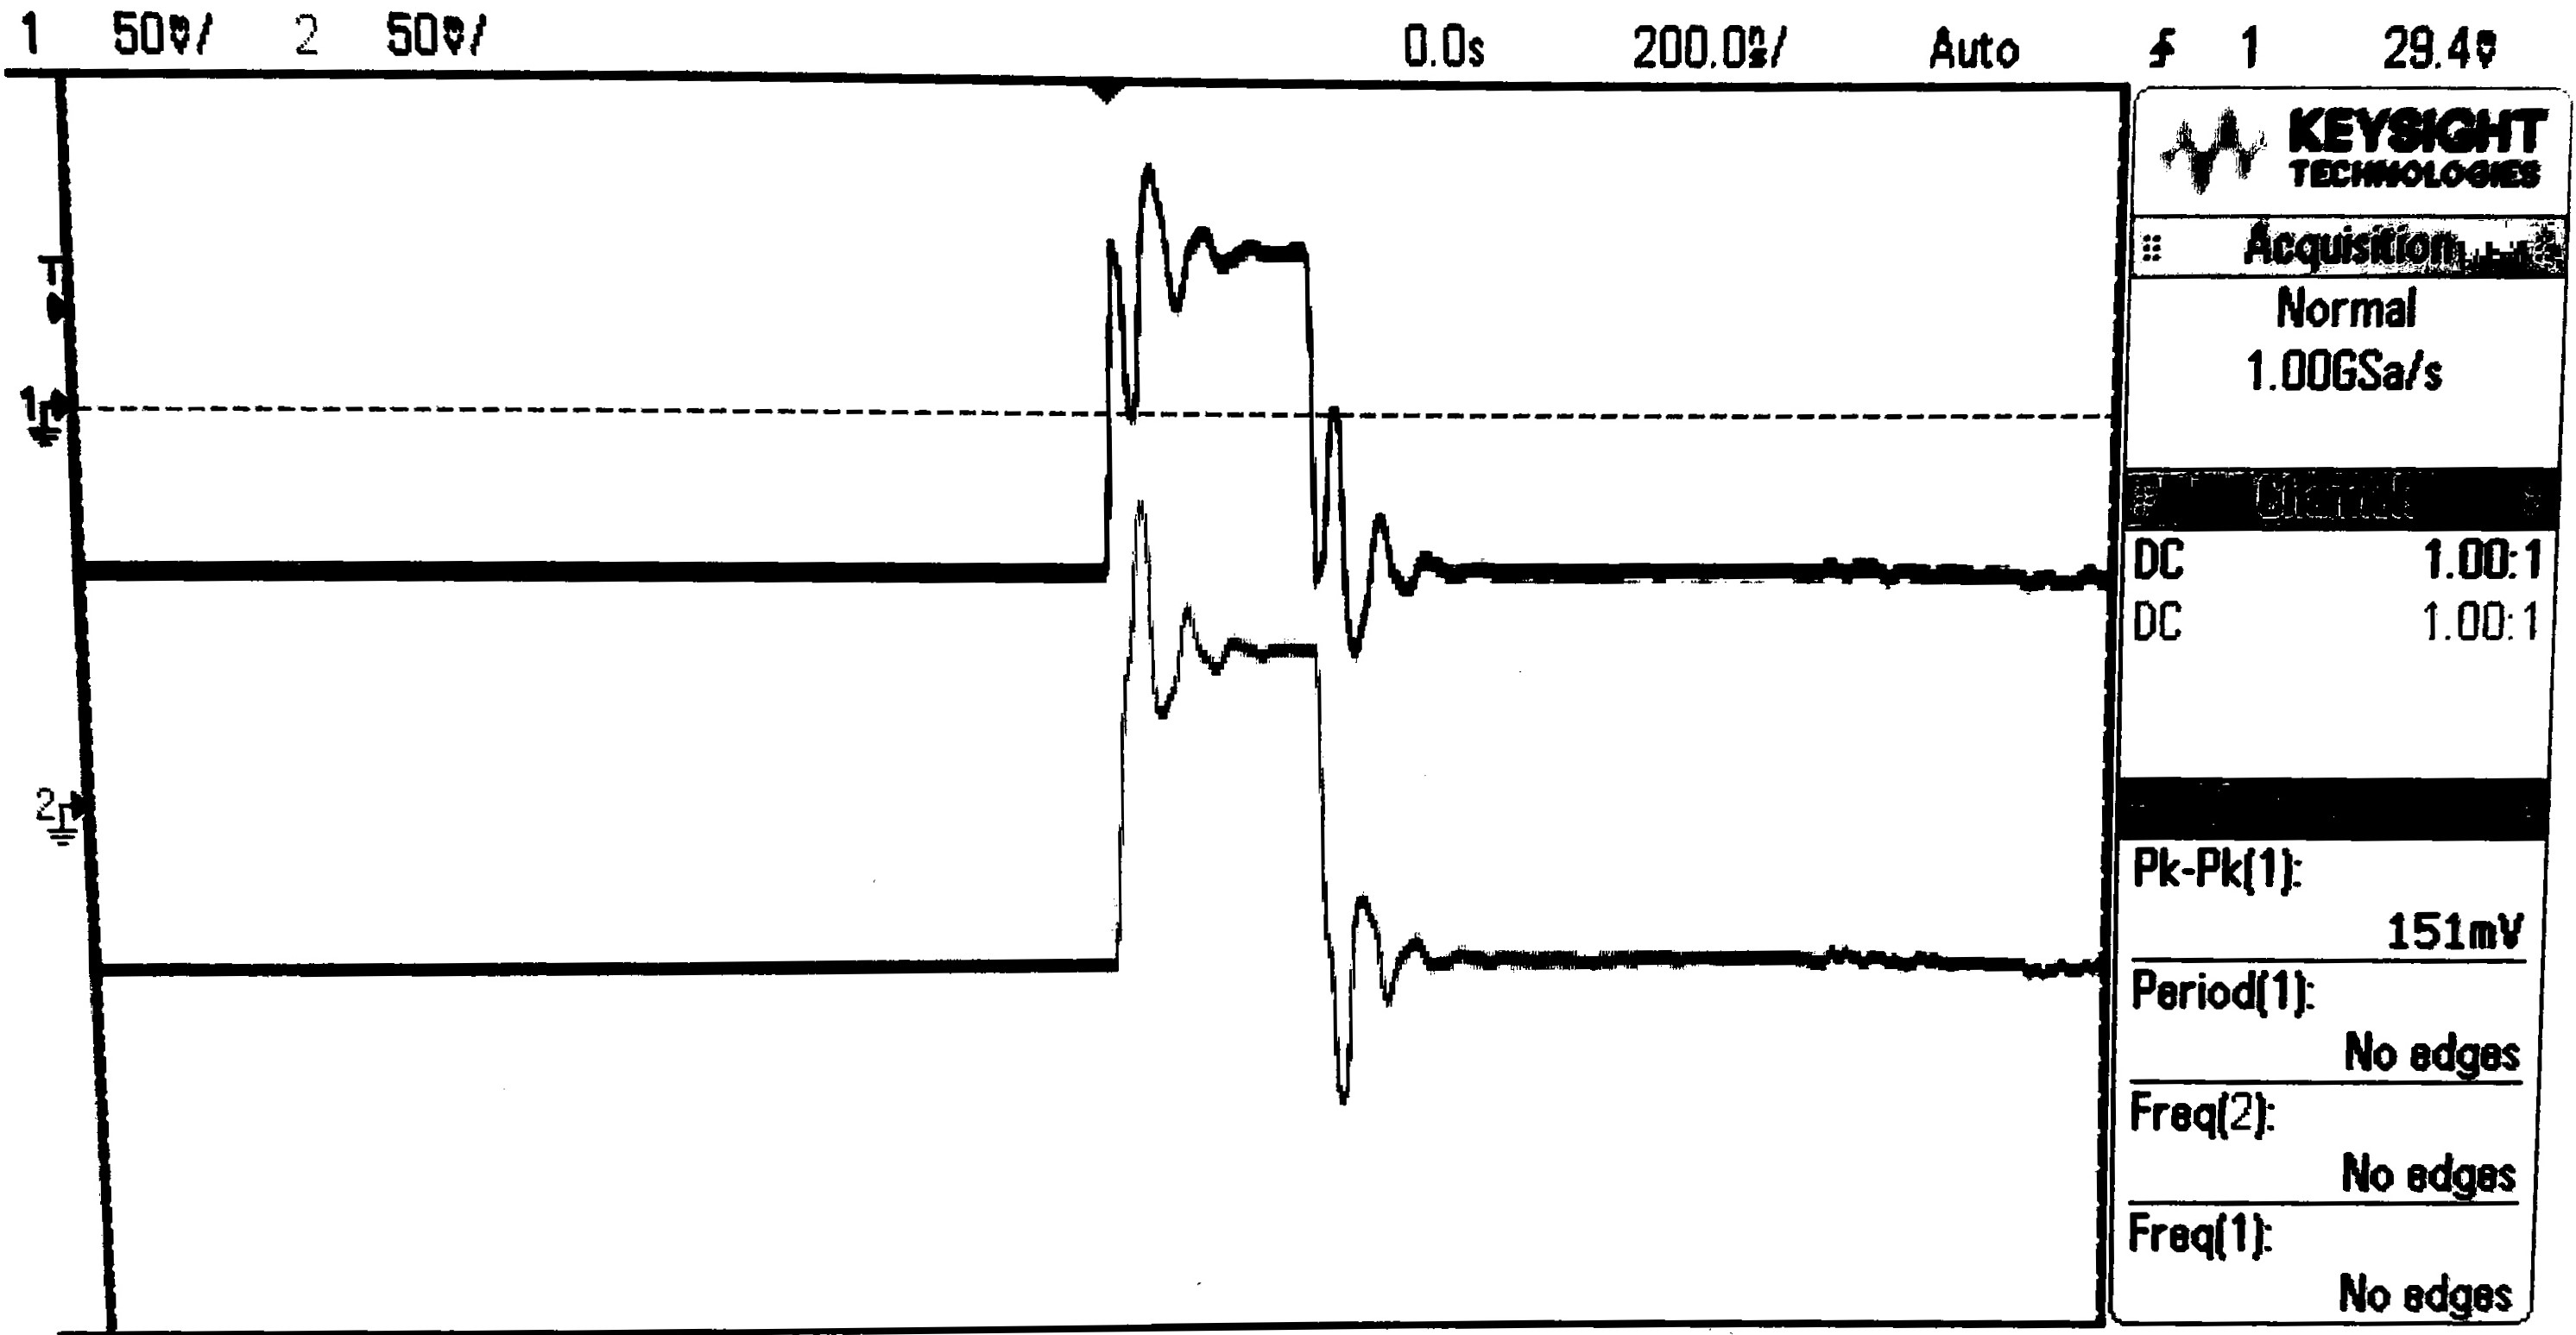
\includegraphics[width=\textwidth]{../photos/lab1/v_t_pt_c.jpg}
        \caption{Port C $(0\text{m})$}
    \end{subfigure}
    \quad
    \begin{subfigure}[b]{0.45\textwidth}
        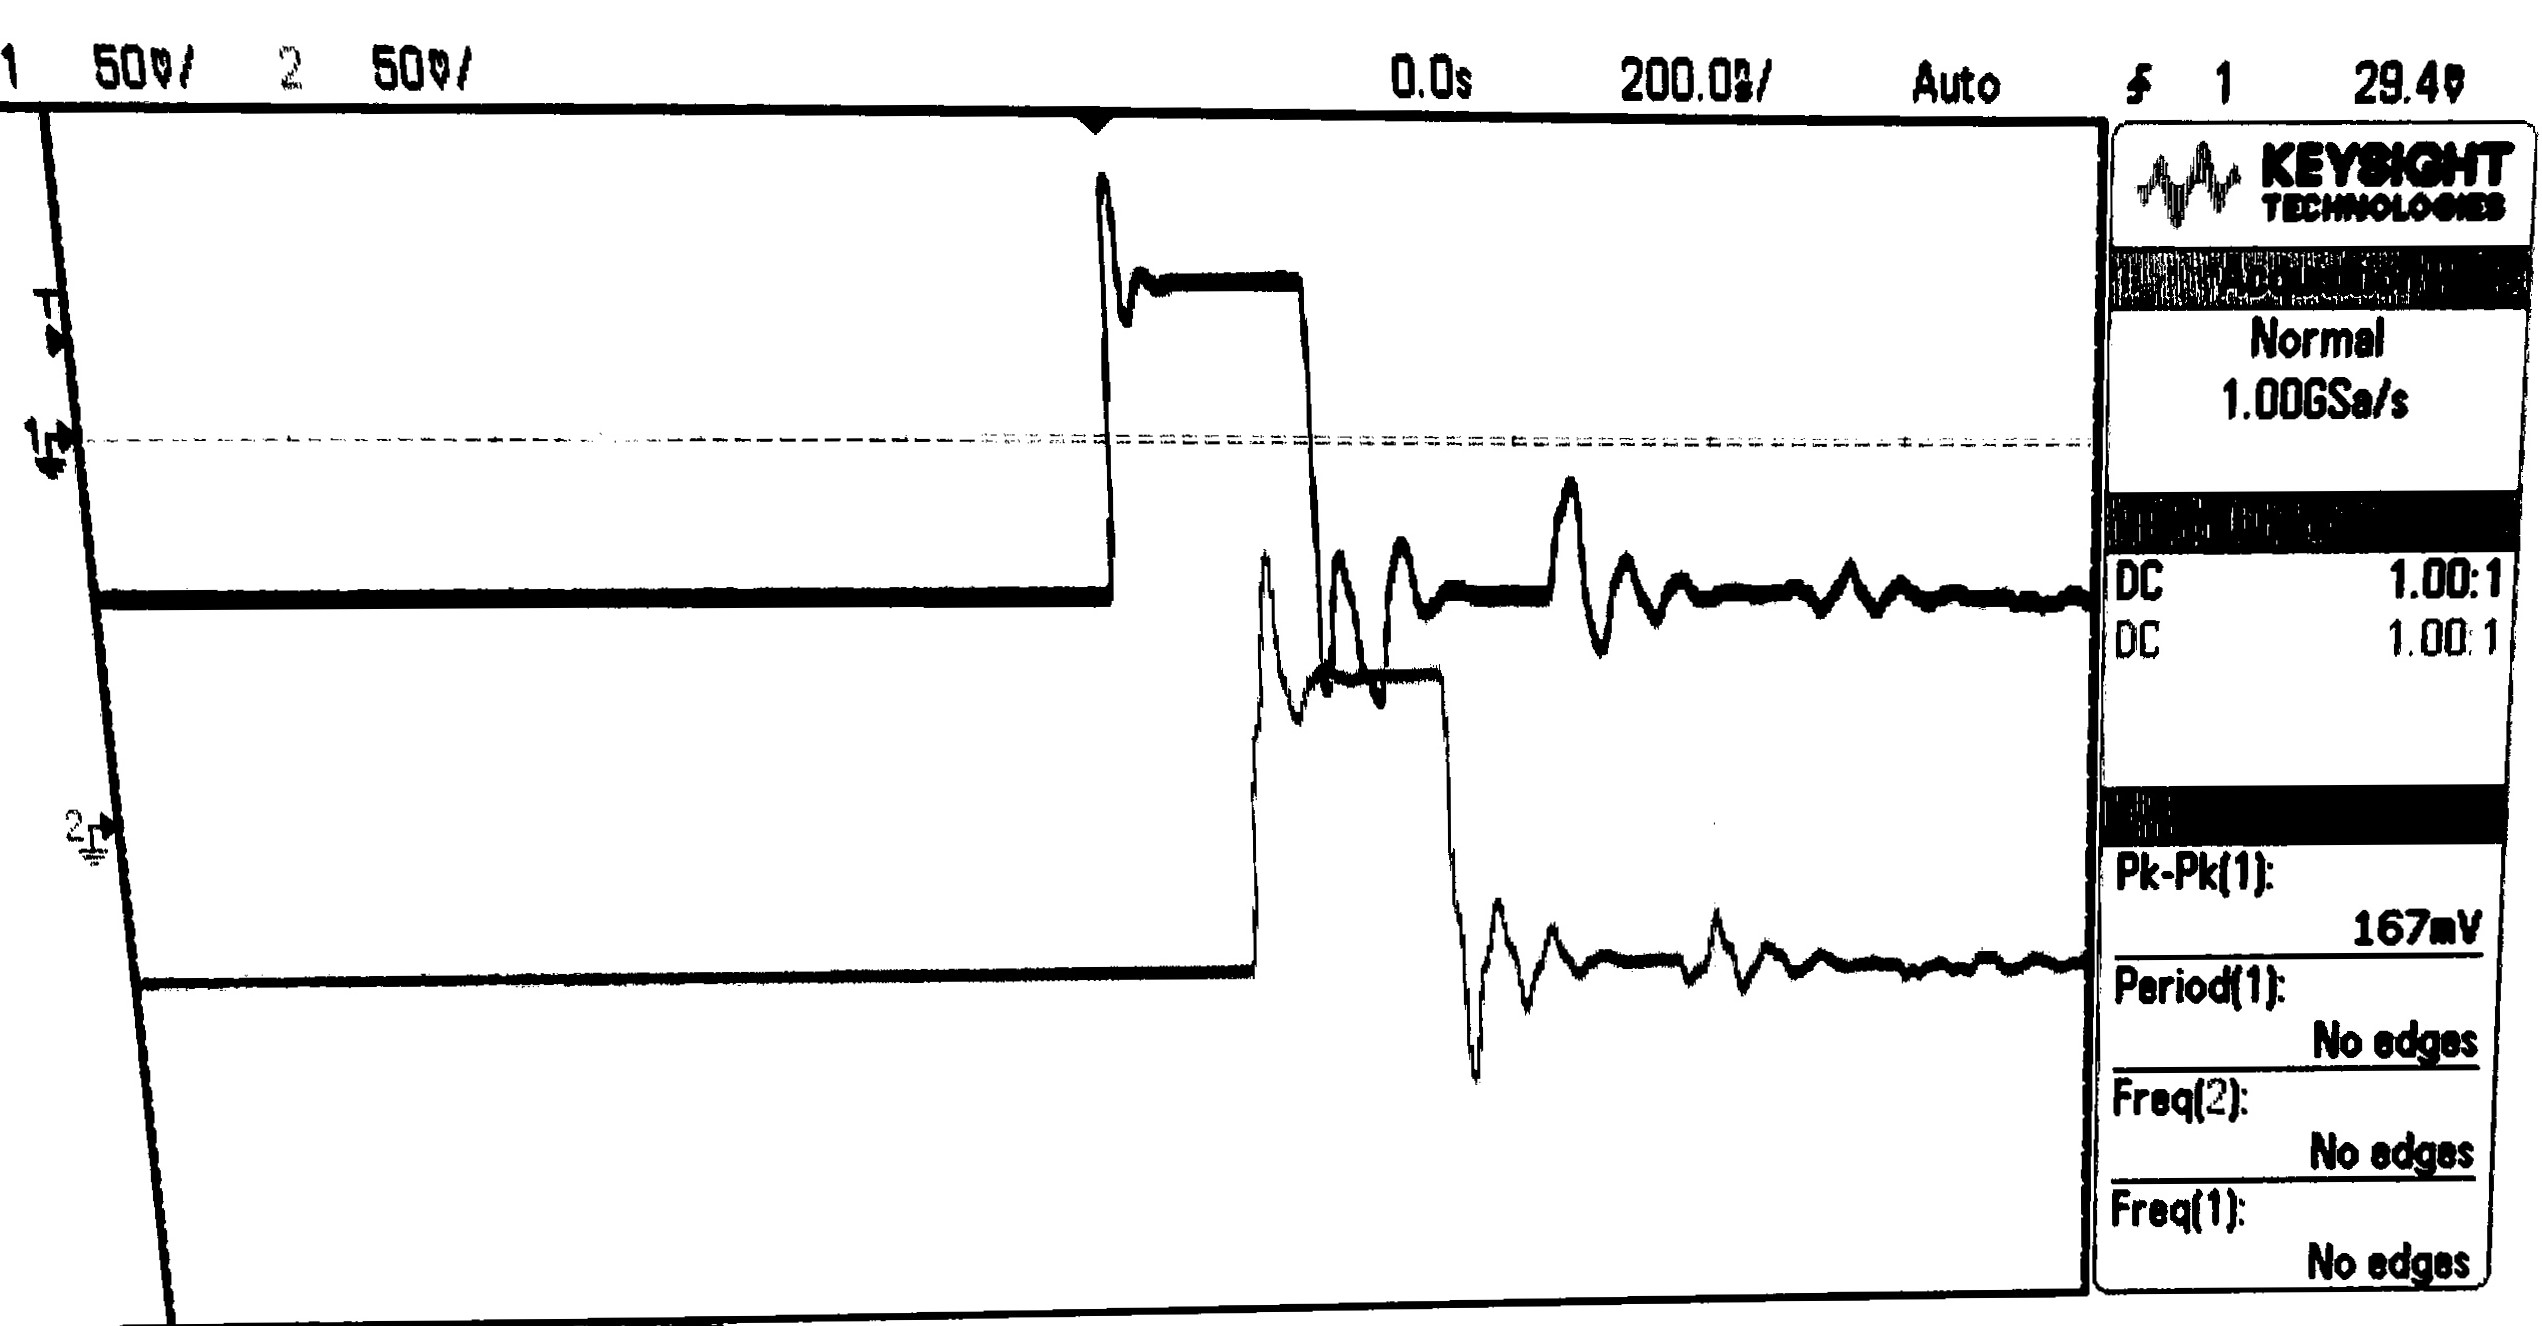
\includegraphics[width=\textwidth]{../photos/lab1/v_t_pt_d.jpg}
        \caption{Port D $(30\text{m})$}
    \end{subfigure}
    \begin{subfigure}[b]{0.45\textwidth}
        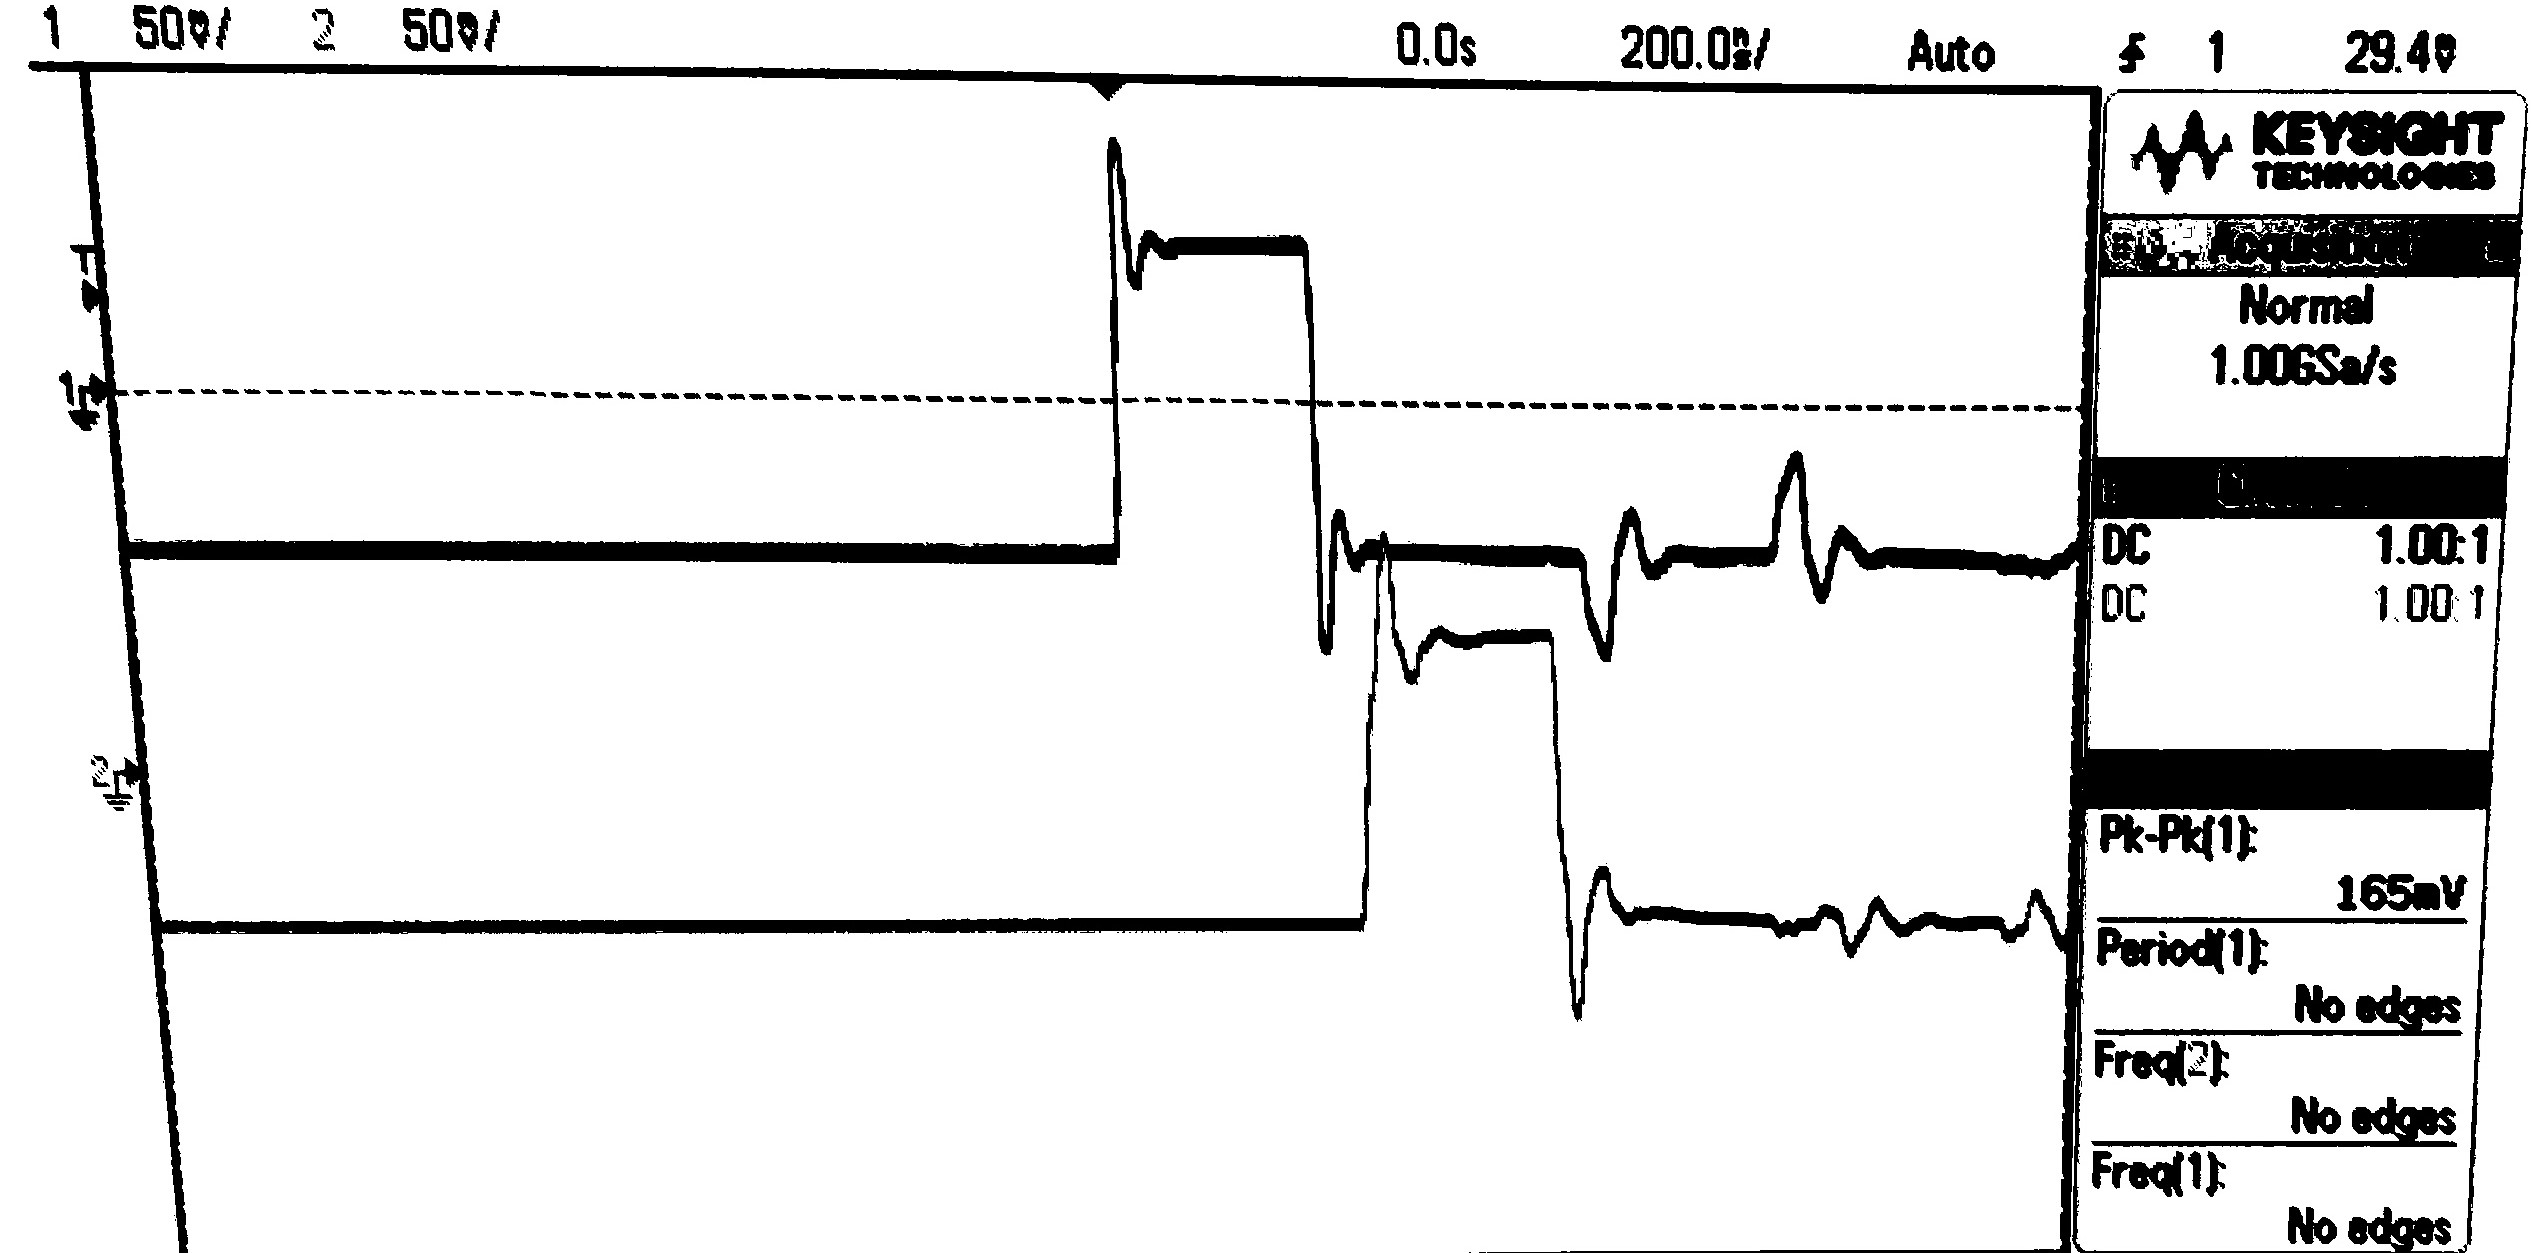
\includegraphics[width=\textwidth]{../photos/lab1/v_t_pt_e.jpg}
        \caption{Port E $(60\text{m})$}
    \end{subfigure}
    \quad
    \begin{subfigure}[b]{0.45\textwidth}
        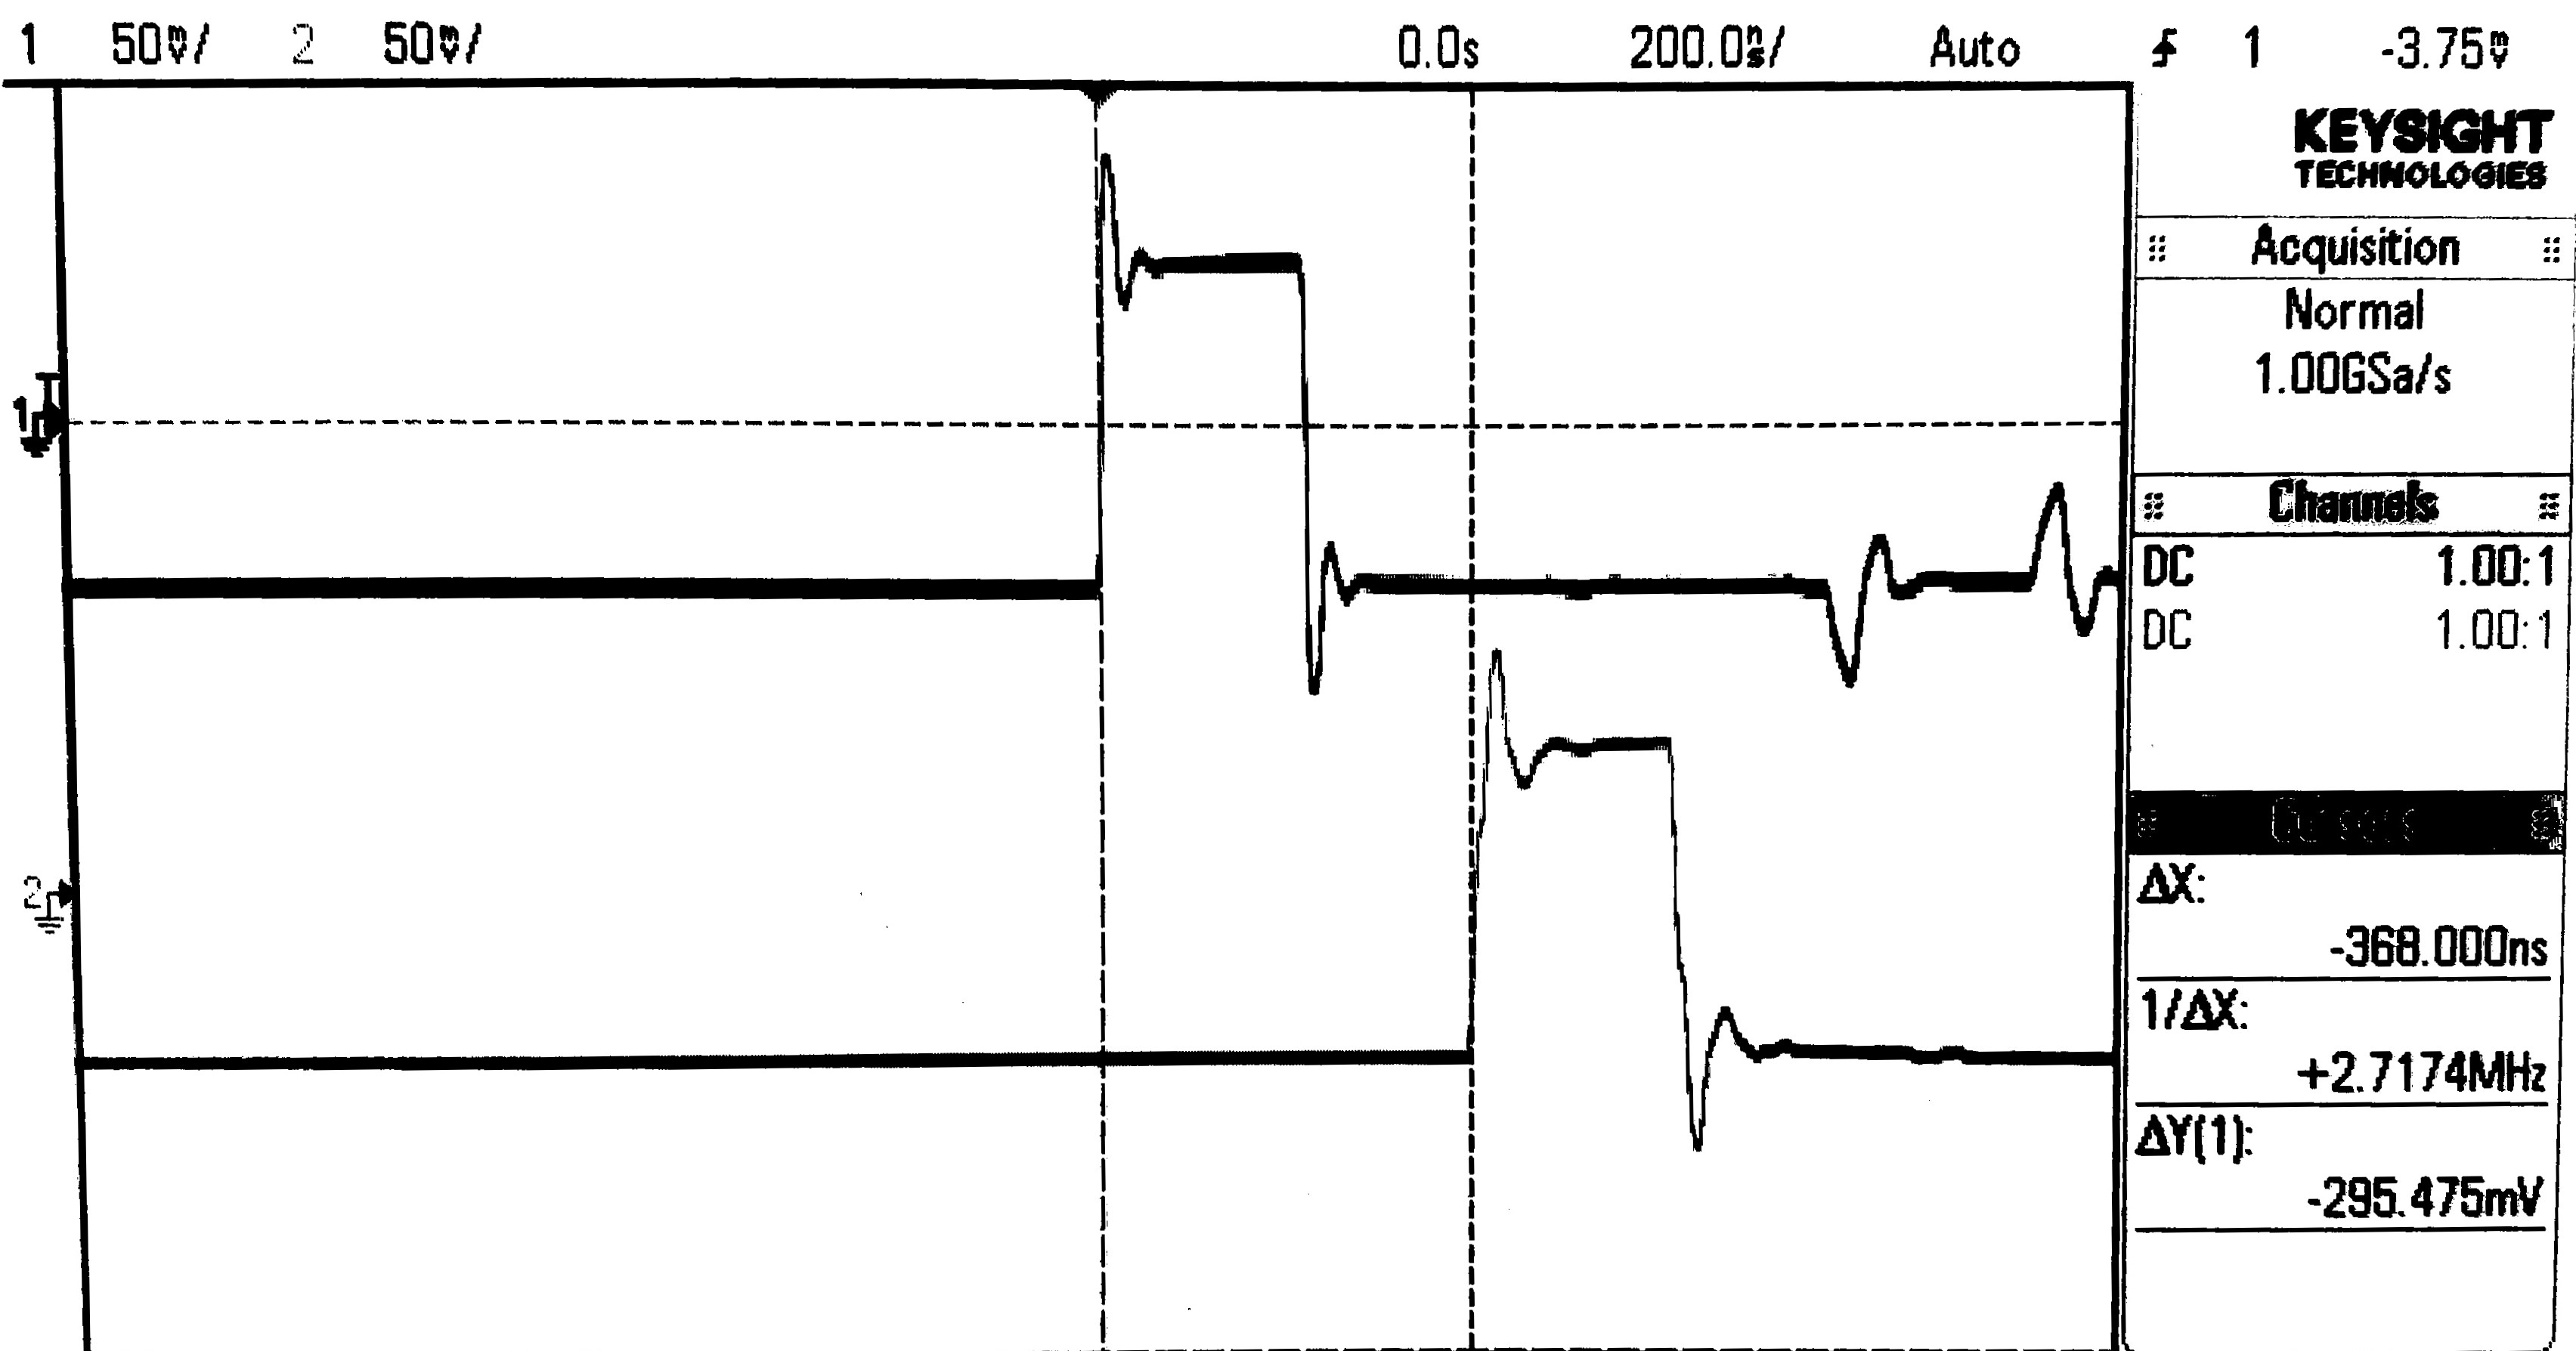
\includegraphics[width=\textwidth]{../photos/lab1/v_t_pt_f.jpg}
        \caption{Port F $(90\text{m})$}
    \end{subfigure}
    \caption{Measured $V(t)$ at different loactions along the transmission line with $Z_L = Z_0$ \vspace{-0.5cm}}
    \label{v_t_matched_tline}
\end{figure}

The recorded time delays, $\Delta t$, relative to the input signal are listed in Table 1.

\begin{table}[h]
    \[
        \begin{array}{c|c}
            \textbf{Port} & \Delta t \textbf{ (ns)} \\ \hline
            \text{D} & 130\\
            \text{E} & 244\\
            \text{F} & 368
        \end{array}
    \]
    \caption{Recorded time delay at different locations along the transmission line\vspace{-0.5cm}}
\end{table}

\section{Determining Velocity of Propagation}

The velocity of propagation of the signal can be calculated by the relation $v_p = \frac{\Delta L}{\Delta t}$, given that
we are able to track the same point on the waveform. Using the data from Table 1,
we get that the average velocity of propagation is $v_{p, \text{avg}} = 2.44 \cdot 10^8 \text{m/s}$.

Now, to find the relative permittivity, we also know that the phase velocity of an electromagentic wave in an electrical transmission line with magnetic permeability, $\mu \approx \mu_0$,
and electric permittivity, $\epsilon = \epsilon_r \epsilon_0$,  is given by: 

\[
    v_p = \frac{1}{\sqrt{\mu \epsilon}} \implies \frac{v_p}{c} \approx 
    \sqrt{\frac{\mu_0\epsilon_0}{\mu_0\epsilon_0\epsilon_r}} \implies 
    \epsilon_r \approx \frac{c^2}{v_p^2} \approx 1.51
\]

The theoretical $V(t)$ plots in Figure 6 closely match the observations in Figure 5.

\begin{figure}[h]
    \centering
    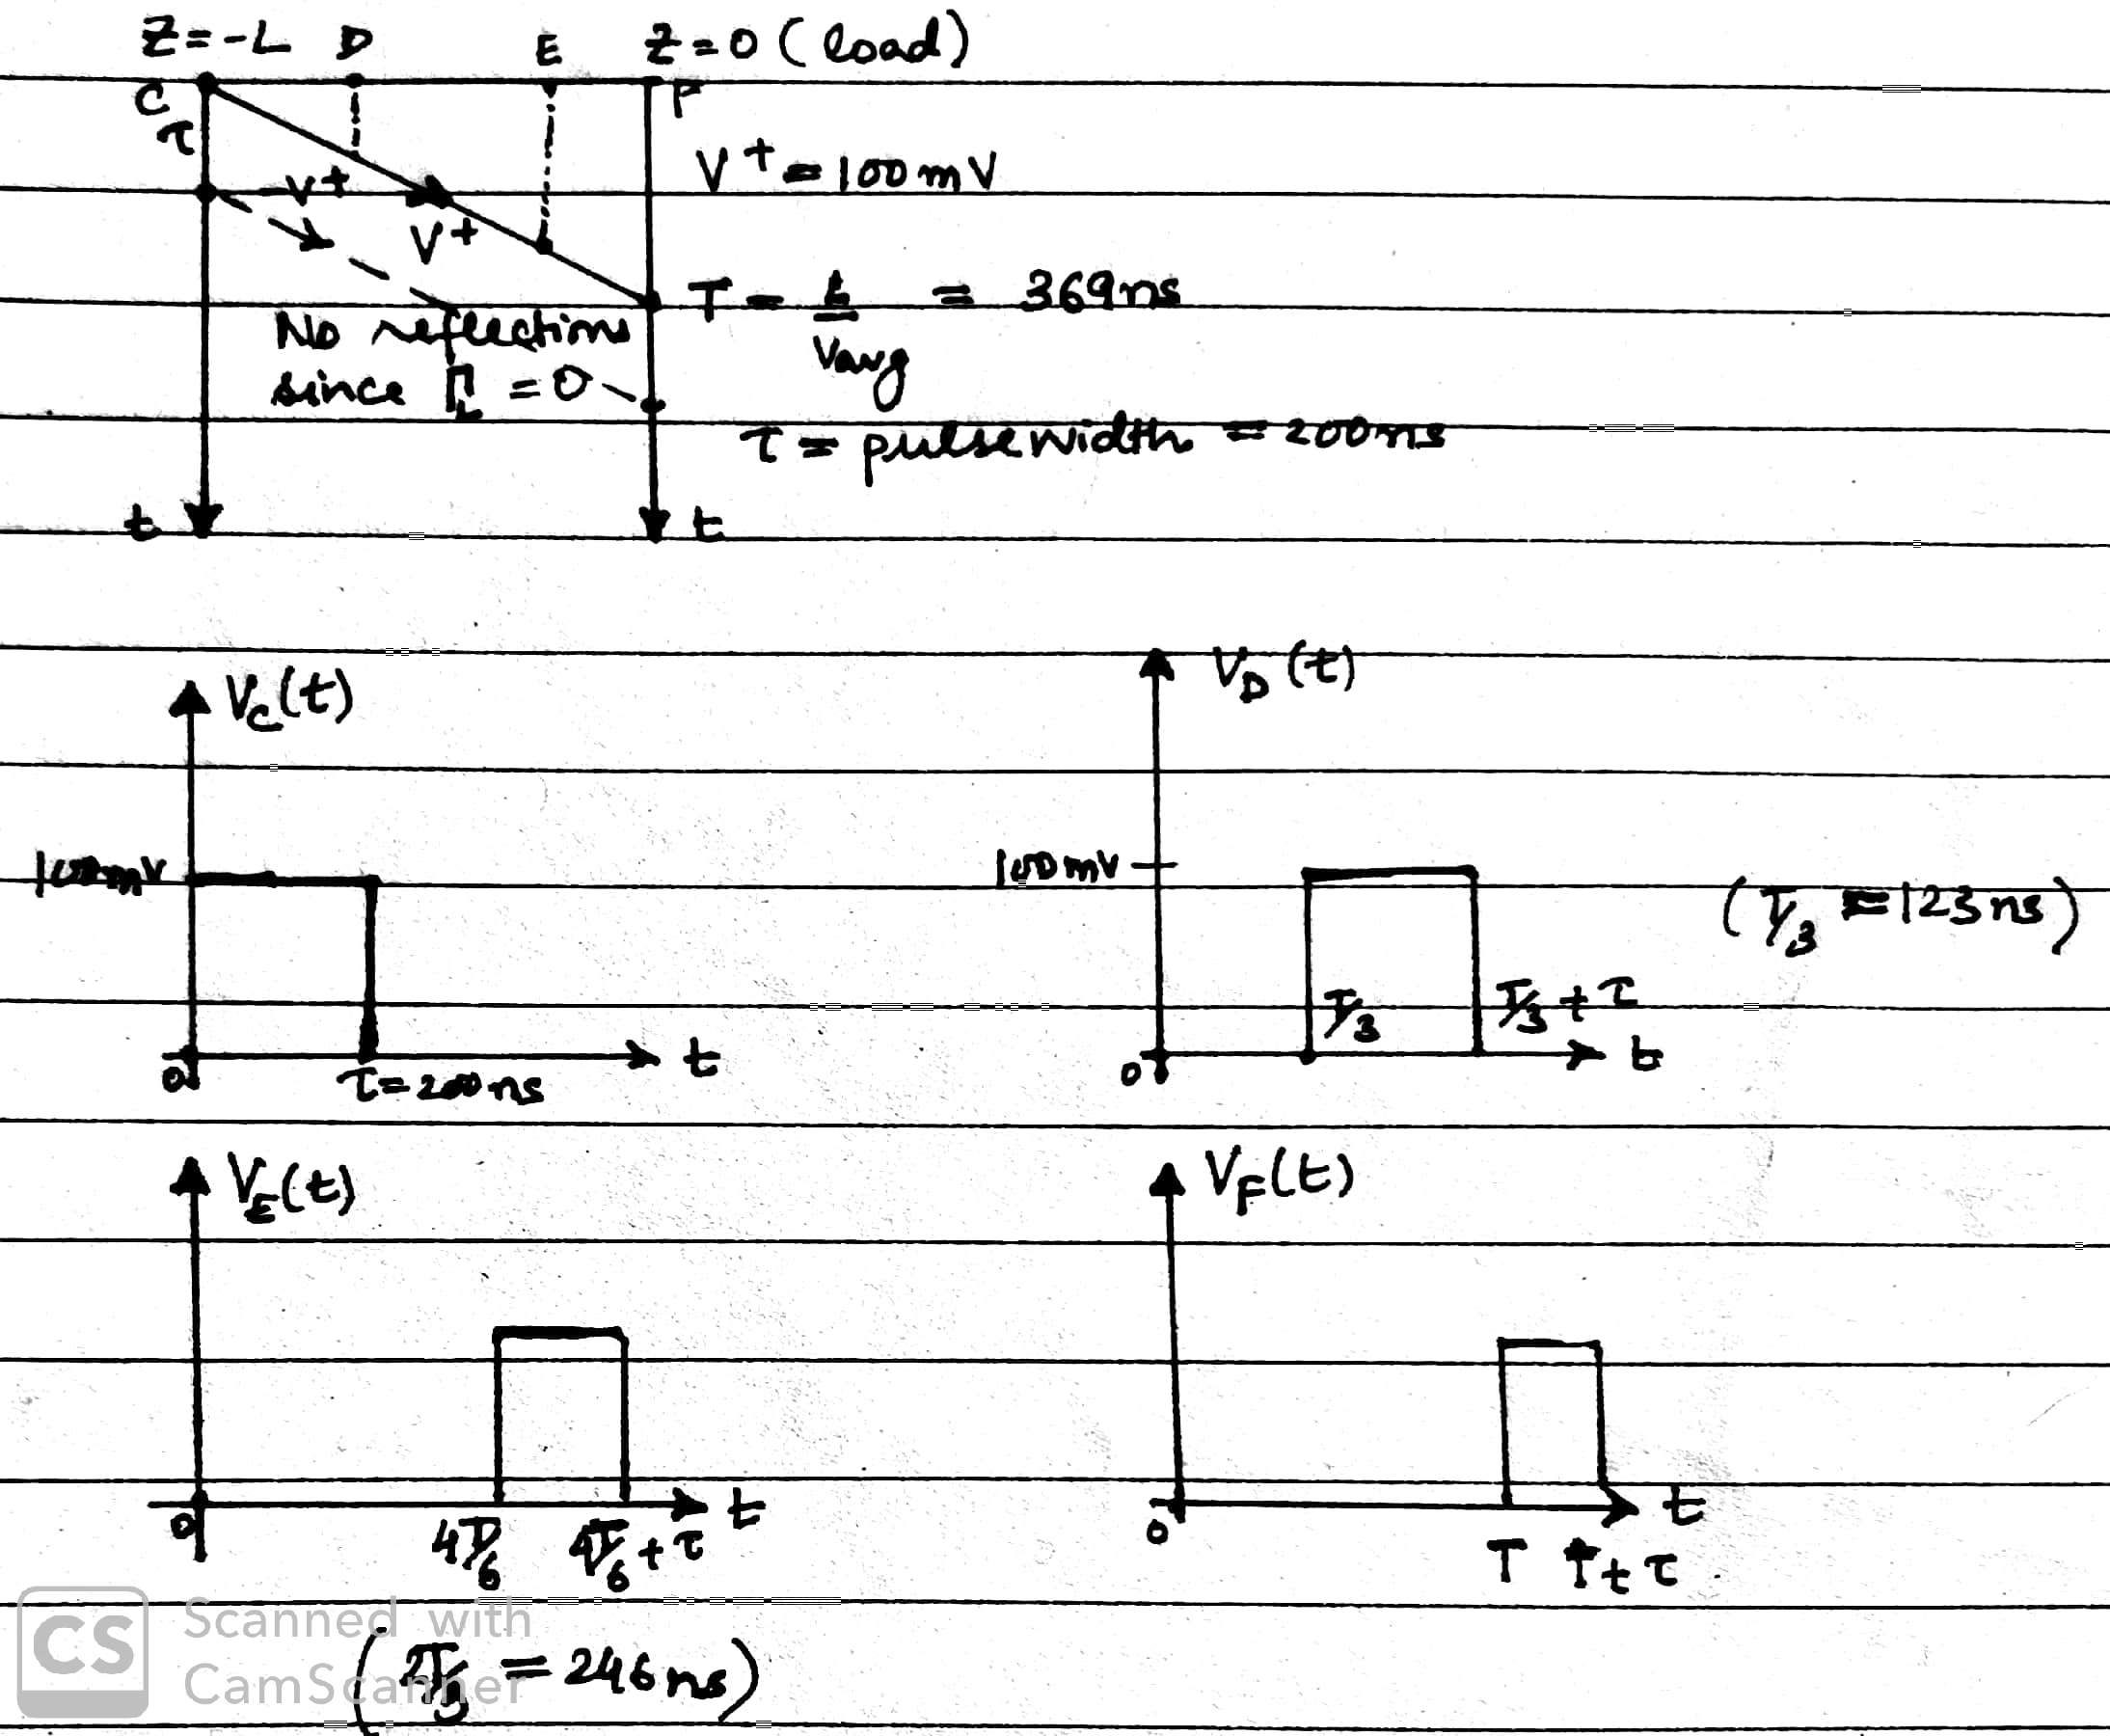
\includegraphics[width=0.45\textwidth]{../photos/lab1/v_t_bounce_no_reflection.jpg}
    \caption{Theoretical bounce diagram and $V(t)$ plots along the transmission line\vspace{-0.5cm}}
    \label{v_t_bounce_no_reflection}
\end{figure}

\section{Simple Reflection}

There is a load mismatch if $Z_L \neq Z_0$ and we know that, in this case, reflection of current and
voltage occurs at the load, i.e. $\tilde v^- \neq 0$ and $\tilde I^- \neq 0$. The load reflection coefficient, $\Gamma_L$,
if defined as:
\[
    \Gamma_L := \frac{\tilde V^-}{\tilde V^+} = \frac{Z_L - Z_0}{Z_L + Z_0}
\]

Thus, in cases where there is a load mismatch, $\Gamma_L \neq 0$, there will be a relection of intensity $\tilde V^- = \Gamma_L\tilde{V^+}$ along the 
transmission line towards the generator and the steady state for a step input will be achieved after the voltage and current 
wave has travelled back and forth once, and this can also be verified using a bounce diagram. The Theoretically for $Z_L = 100\Omega$, $\Gamma_L = \frac{50\Omega}{150\Omega} = \frac{1}{3} $ and through the measurements, we observe the reflection 
coefficient $\Gamma_L = \frac{30\text{mV}}{100\text{mV}} = \frac{3}{10} \approx \frac{1}{3}$.

The measurements for reflected voltage waves can be found in Figure 7. Channel 1 (top) waveform has been 
recorded at port C ($0\text{m}$) and channel 2 (bottom) waveform has been recorded at port F ($90\text{m}$).
The pulsewidth $\tau$ of the signal was set such that it was equal to the time delay $T$ for a pulse to reach
port F from port C, which made the signal recordings at port C and F exactly out of phase. In terms of magnitude, the
signal at port F was a superposition of the incident and reflected wave $\tilde V_F = \tilde V^+ + \Gamma_L\tilde V^+$.
Similarly at port C, the signal at $t \in (2T, 3T)$, $\tilde V_C = \Gamma_L\tilde V^+ = \tilde V^-$, which can all again
be verified using a bounce diagram. The theoretical $V(d)$ graphs for different time points can be found in Figure 8.

\begin{figure}[ht]
    \centering
    \begin{subfigure}[b]{0.45\textwidth}
        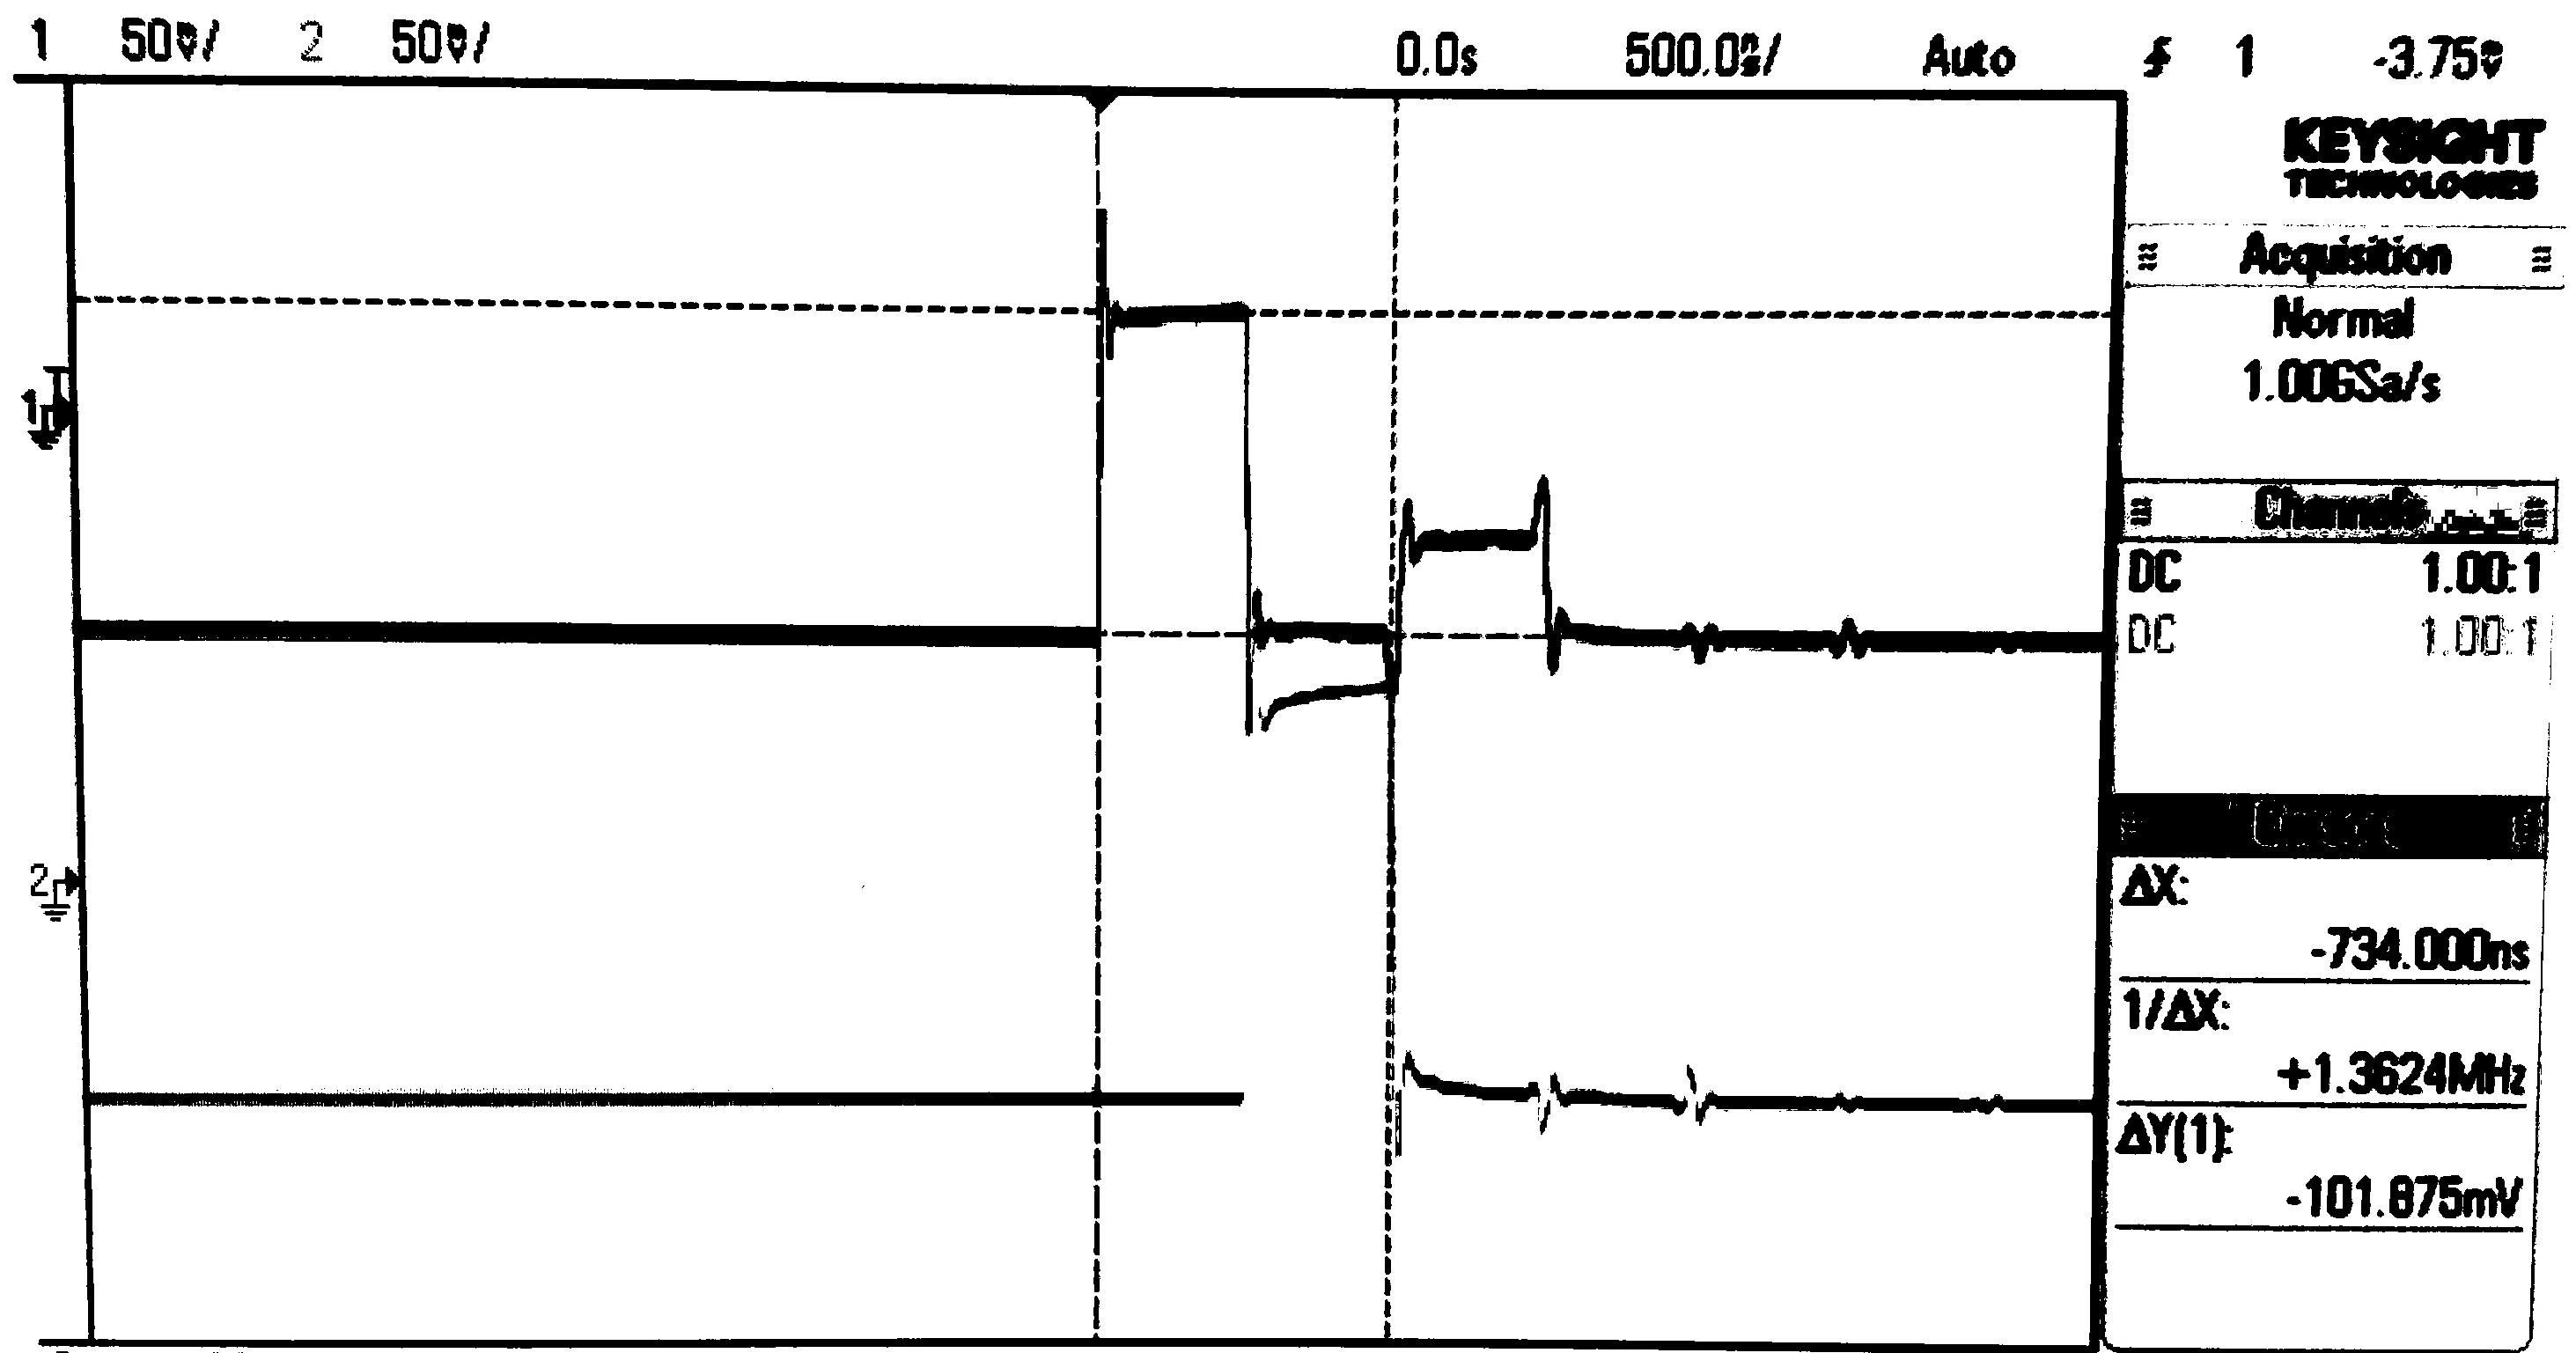
\includegraphics[width=\textwidth]{../photos/lab1/v_t_gamma_L_1.jpg}
        \caption{$\tilde V_1 = \tilde V^+ \approx 100\text{mV}$}
    \end{subfigure}
    \quad
    \begin{subfigure}[b]{0.45\textwidth}
        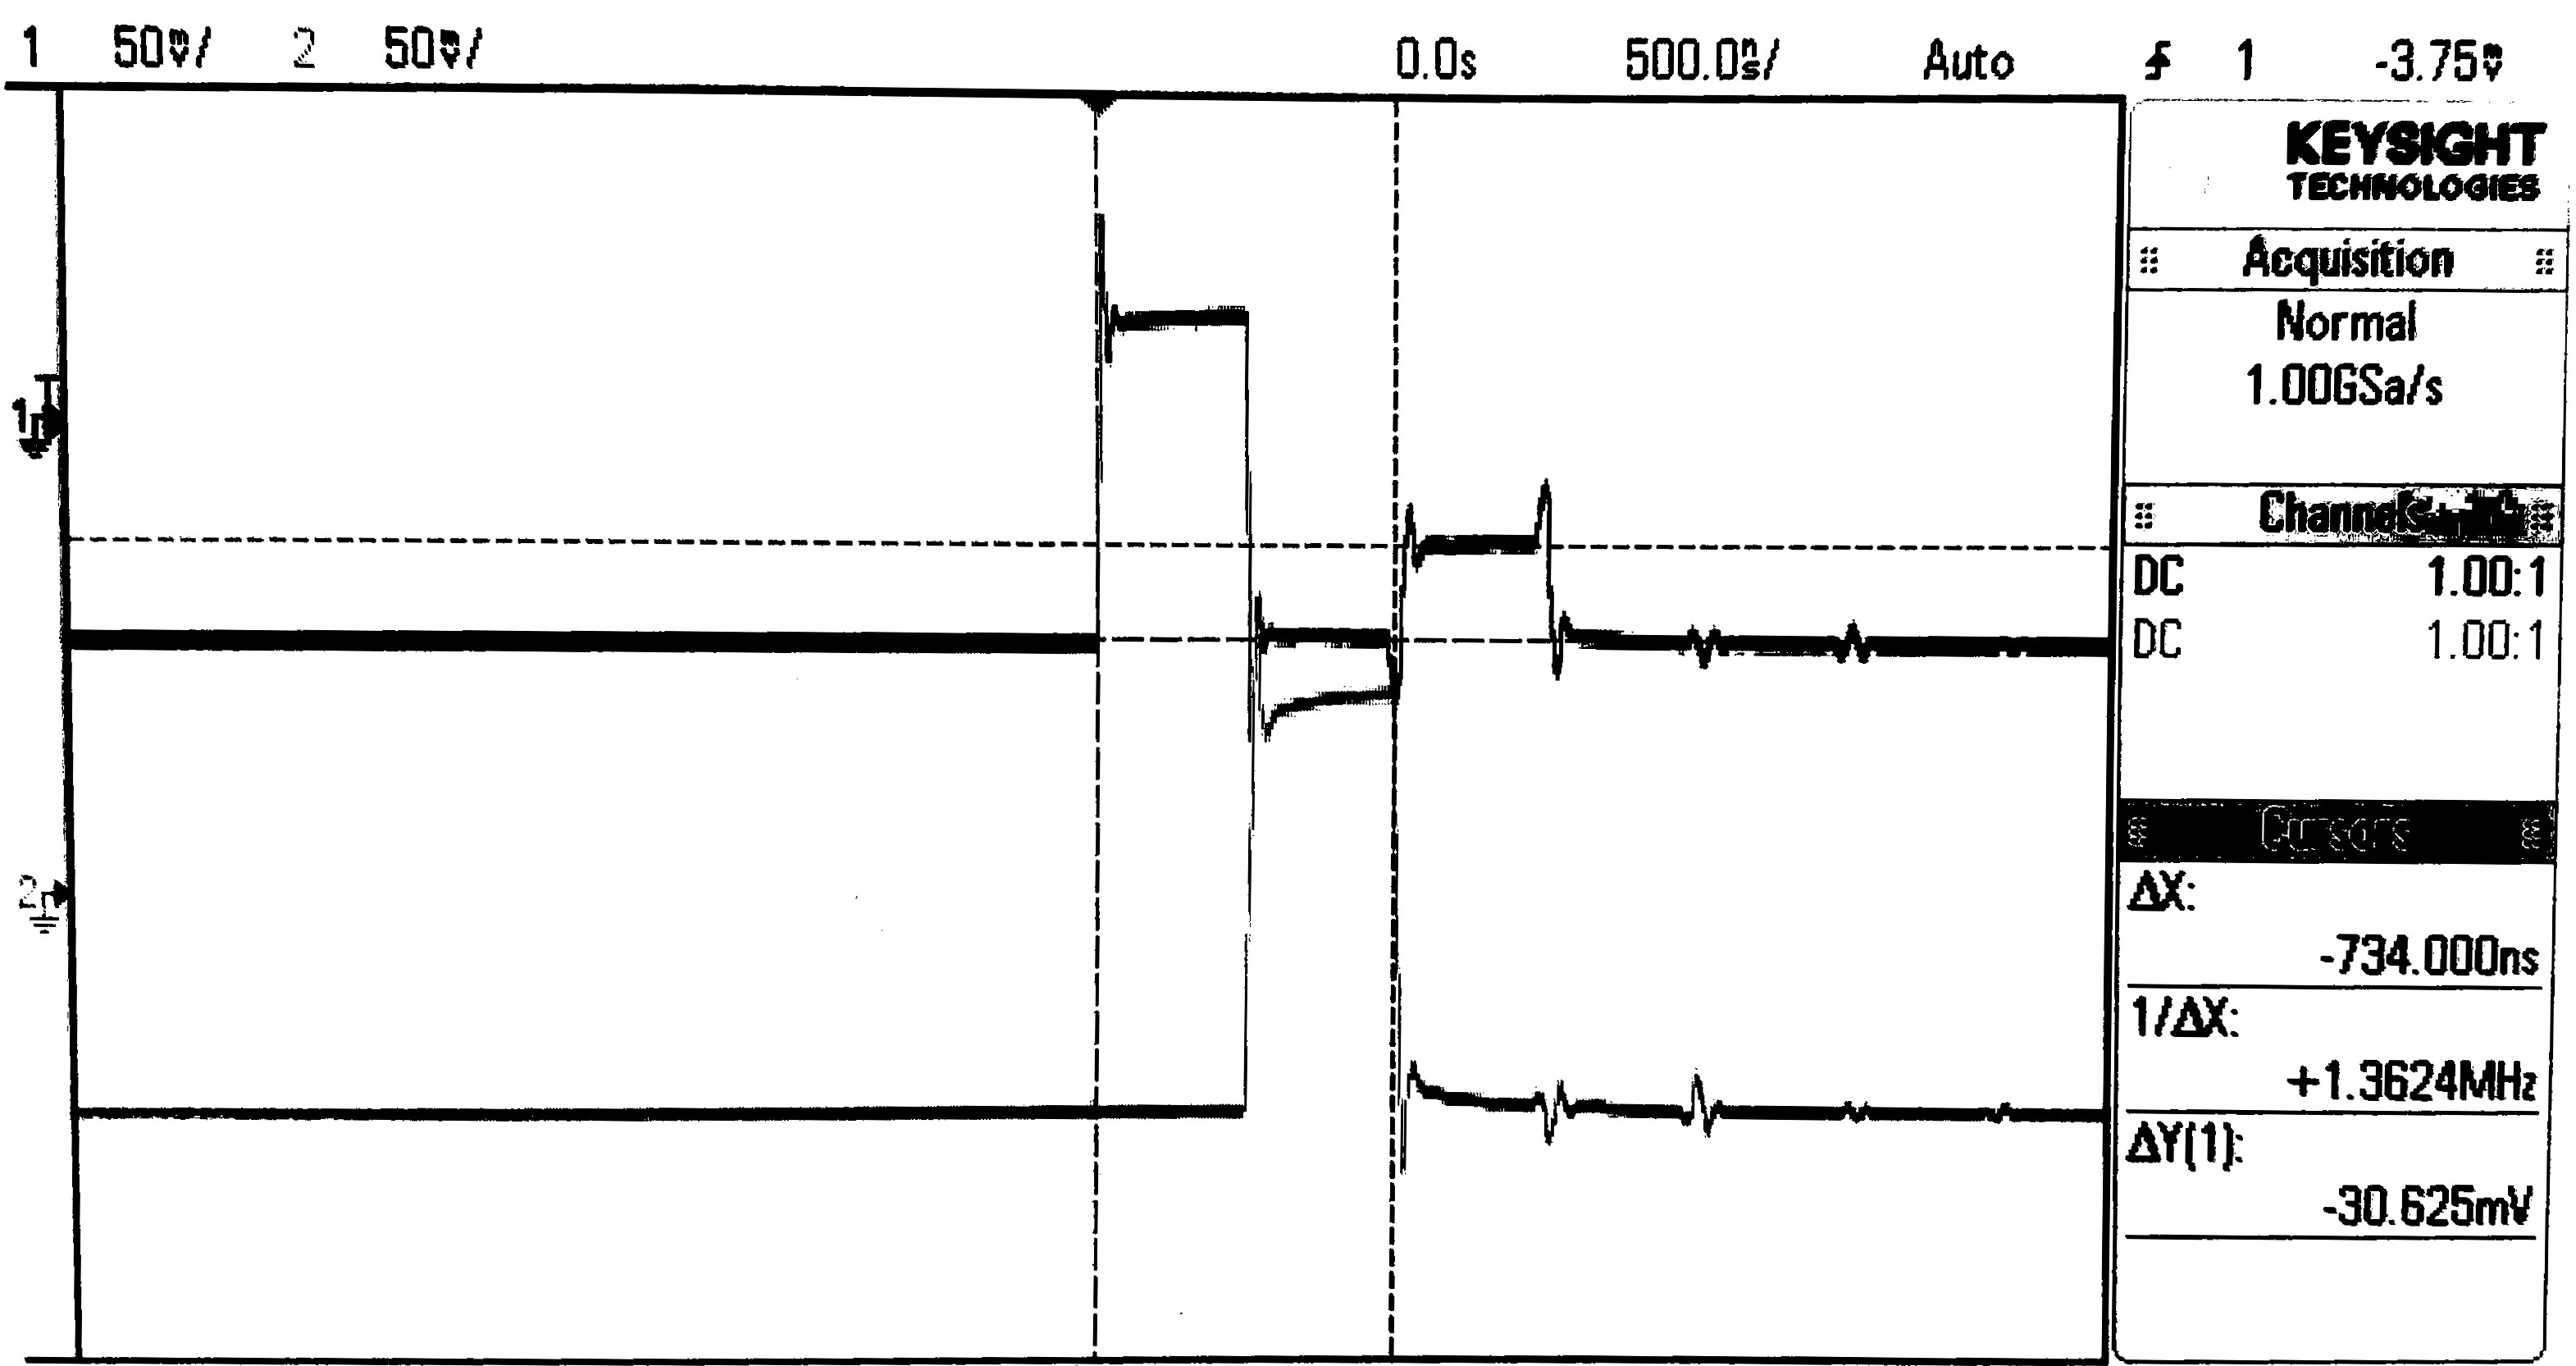
\includegraphics[width=\textwidth]{../photos/lab1/v_t_gamma_L_2.jpg}
        \caption{$\tilde V_2 = \Gamma_L\tilde V^+ = \tilde V^- \approx 30\text{mV}$}
    \end{subfigure}
    \caption{$\tilde V$ measured at port C and port F for input signal with pulsewidth $\tau = T$\vspace{-0.5cm}}
    \label{v_t_c_f}
\end{figure}

\begin{figure}[h]
    \centering
    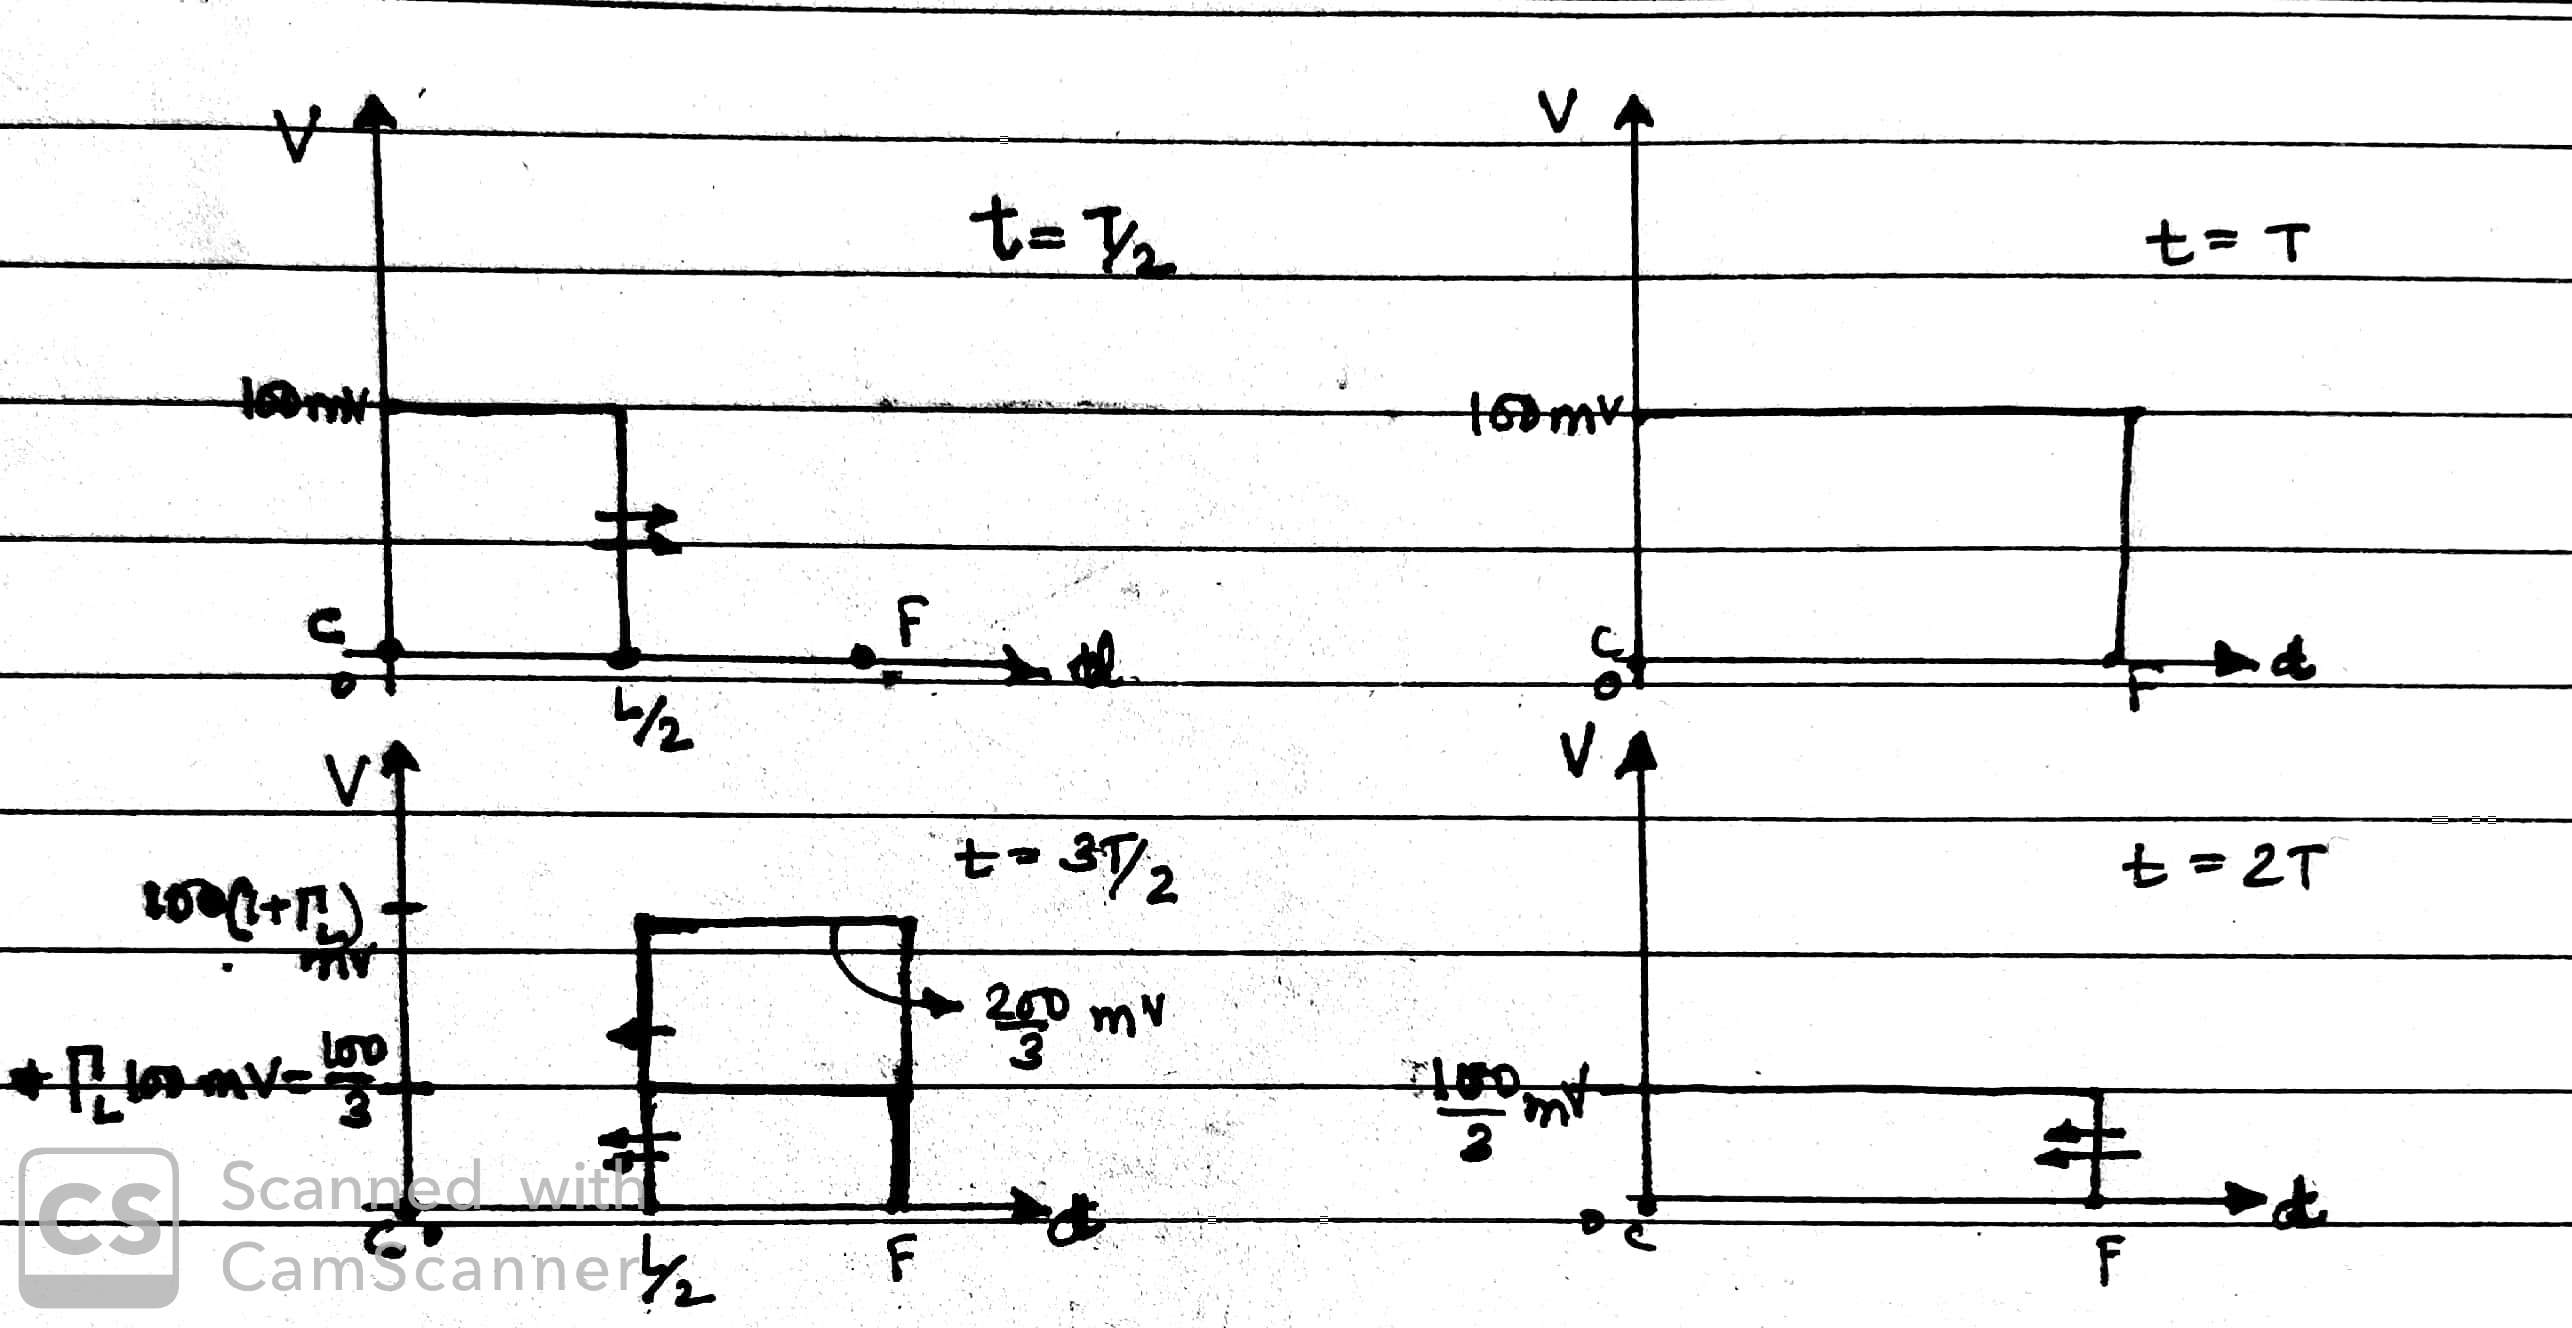
\includegraphics[width=0.45\textwidth]{../photos/lab1/v_d_gamma_L.jpg}
    \caption{$V(d)$ plots at different time points\vspace{-0.5cm}}
    \label{v_d_different_T}
\end{figure}

\section{Multiple Reflections}

For mismatched generator side, $Z_g = 150\Omega$, as well as the load side, $Z_L = 20\Omega$, there will 
be reflections on both ends of the transmission line. 

\section{Input Impedance and Transmission Line Length}

\begin{figure}[h] \centering
    \begin{circuitikz} 
        \draw
        (0, 2) to [V, l_=$\tilde V_g$] (0, 0) -- (2, 0)
        to [R, l_=${Z_{\text{in}}}$, -*] (2, 2)
        to [R, l_=$Z_g$] (0, 2);

        \draw (2, 2) -- (2.25, 2.25);
        
        \draw 
        (3.45, 2.4) 
        node[]{$\displaystyle{\tilde V_{\text{in}} = \tilde V_g\frac{Z_{\text{in}}}{Z_{\text{in}} + Z_g}}$} 
        (3.45, 2.4);
    \end{circuitikz}
    \caption{Voltage division over net input impedance, $Z_\text{in}$\vspace{-0.5cm}}
    \label{volt_diag}
\end{figure}

We know that the impedance changes.

\[
    Z_{\text{in}} = Z(z)\big\rvert_{z=-L} = Z_0 \frac{1+\Gamma e^{j2\beta z}}{1-\Gamma e^{j2\beta z}}\bigg\rvert_{z=-L} = Z_0 \frac{Z_L + jZ_0\tan{\beta L}}{Z_0 + jZ_L\tan{\beta L}}
\]

\section{Conclusion}

Through this lab, 

\section{Notes}

All images taken during the lab were post-processed in a batch using a custom script
that bit-wise inverts the pixels and binarizes the resulting image based on a custom threshold.
No adjustments or modifications were made to the readings, for which the oscilloscope's measurements
are also shown alongside the waveforms. All scripts and related work can be found at 
\href{https://github.com/pranshumalik14/ece320-labs}{\texttt{github.com/pranshumalik14/ece320-labs}}.

\end{document}